\documentclass[a4paper]{article}
\usepackage[spanish]{babel}
\usepackage[utf8]{inputenc}
\usepackage{graphicx}
\usepackage{pdfpages}
\usepackage{enumerate}
\usepackage{listings}
\usepackage{color}
\usepackage{indentfirst}
\usepackage{fancyhdr}
\usepackage{latexsym}
\usepackage[colorlinks=true, linkcolor=black]{hyperref}
\usepackage{wrapfig}
\usepackage{algpseudocode}
\usepackage{calc}
\usepackage{amsmath, amsthm, amssymb}
\usepackage{amsfonts}
\usepackage{lscape}
\usepackage{float}
\usepackage{hyperref}
\definecolor{gray}{gray}{0.5}
\definecolor{light-gray}{gray}{0.95}
\definecolor{orange}{rgb}{1,0.5,0}

\usepackage{fancyhdr}
\pagestyle{fancy}

%\renewcommand{\chaptermark}[1]{\markboth{#1}{}}
\renewcommand{\sectionmark}[1]{\markright{\thesection\ - #1}}

\fancyhf{}

\fancyhead[LO]{Sección \rightmark} % \thesection\
\fancyfoot[LO]{\small{Leandro Matayoshi, Matías Pizzagalli, Gastón Requeni, Martín Santos}}
\fancyfoot[RO]{\thepage}
\renewcommand{\headrulewidth}{0.5pt}
\renewcommand{\footrulewidth}{0.5pt}
\setlength{\hoffset}{-0.8in}
\setlength{\textwidth}{16cm}
%\setlength{\hoffset}{-1.1cm}
%\setlength{\textwidth}{16cm}
\setlength{\headsep}{0.5cm}
\setlength{\textheight}{25cm}
\setlength{\voffset}{-0.7in}
\setlength{\headwidth}{\textwidth}
\setlength{\headheight}{13.1pt}

\renewcommand{\baselinestretch}{1.1}  % line spacing


\usepackage{underscore}
\usepackage{caratula}
\usepackage{url}

\newcommand{\cod}[1]{{\tt #1}}
\newcommand{\negro}[1]{{\bf #1}}
\newcommand{\ital}[1]{{\em #1}}
\newcommand{\may}[1]{{\sc #1}}
\newcommand{\tab}{\hspace*{2em}}

\newcommand{\sprintstory}[6]{\begin{tabular}{| p{3cm} | p{12cm} |}
 \hline
 TargetProcess ID: & #1 \\
 \hline
 User Story: & #2 \\
 \hline
 Esfuerzo estimado: & #3 \\
 \hline
 Business Value: & #4 \\
 \hline
 Descripción: & #5 \\
 \hline
 Criterios de\newline Aceptación: & #6 \\
 \hline
\end{tabular}}

\newcommand{\usecase}[3]{\noindent\textbf{CU\##1. #2}\\
#3\\
~\\
}

\newenvironment{taskstable}
{ \begin{tabular}{| p{14cm} | p{1cm} |}
 \hline
 \multicolumn{2}{|c|}{{\bf División en tareas}}\\
 \hline
 {\bf Tarea} & {\bf HH}\\
 \hline }
{ \end{tabular} }

\newcommand{\task}[2]{#1 & #2\\
 \hline}

\hypersetup{
 pdfstartview= {FitH \hypercalcbp{\paperheight-\topmargin-1in-\headheight}},
 pdfauthor={Grupo},
 pdfsubject={Dise\~{n}o}
}

\lstset{escapechar=@}

\begin{document}

\thispagestyle{empty}
\materia{Ingeniería de Software II}
\submateria{Primer Cuatrimestre de 2016}
\titulo{Trabajo Práctico II: The Curry Game release v7.1.2}

\integrante{Leandro Matayoshi}{79/11}{leandro.matayoshi@gmail.com}
\integrante{Matías Pizzagalli}{257/12}{matipizza@gmail.com}
\integrante{Gastón Requeni}{400/11}{grequeni@hotmail.com}
\integrante{Martín Santos}{413/11}{martin.n.santos@gmail.com}

\makeatletter

\maketitle

\newenvironment{myindentpar}[1]
{\begin{list}{1}
         {\setlength{\leftmargin}{#1}}
         \item[]
}
{\end{list}}

\newcommand{\escenario}[8] {
  \noindent \underline {{#1}} \newline
  \noindent \textit{'{#2}'}
  \begin{itemize}
    \item \textbf{Fuente:} {#3}
    \item \textbf{Estímulo:} {#4}
    \item \textbf{Entorno:} {#5}
    \item \textbf{Artefacto:} {#6}
    \item \textbf{Respuesta:} {#7}
    \item \textbf{Medición de respuesta:} {#8}
  \end{itemize}
}

\newpage
% \section{Casos de uso}
% \begin{enumerate}
  \item Simulando desafío de basket según nuevas reglas
  \item Simulando desafíos de otros deportes
  \item Estableciendo estadísticas de jugadores de sitios oficiales y modificadas según redes sociales
  \item Participando en modo liga de fantasía. Usuario. 
  \item Participando en desafío o torneo grupal. Usuario.
  \item Chateando con otros participantes. Usuario.
  \item Posicionándose en ranking jerárquico. Usuario.
  \item Apostando dinero real en desafíos. Usuario.
  \item Controlando acceso de usuarios según leyes de la región respecto a apuestas online
  \item Mirando desafío ficticio en tiempo real. Usuario.
  \item Mirando en vivo partidos de ligas reales. Usuario.
  \item Agregando publicidad en el sitio
  \item Consultando datos estadísticos de usuarios de la aplicación
\end{enumerate}

\subsection{Descripción de los casos de uso, agrupados por área}

\subsubsection{Simulación}

\textbf{Simulando desafío de basket según las nuevas reglas}

Se refiere a modificar la simulación de forma tal que su duración sea similar a la de un partido real. Además incluye incorporar 
nuevas acciones, eventos y características del entorno que modifican la simulación: fouls, tiros libres, cambio de jugadores, cansancio
por minutos en cancha, estadios locales y visitantes, condiciones climáticas, movimientos de los jugadores y posiciones en cancha.

~

\textbf{Simulando desafíos de otros deportes}

Se refiere a la posibilidad de simular desafíos para diversos deportes

~

\textbf{Estableciendo estadísticas de jugadores de sitios oficiales y modificadas según redes sociales}

Se refiere a levantar las estadísticas de jugadores desde sitios oficiales y autorizados. Además las estadísticas
de los jugadores deberán modificarse en función de las menciones de los jugadores hechas en diversas redes sociales,
incluído el sistema de mensajería entre participantes.

\subsubsection{Desafíos}

\textbf{Participando en modo liga de fantasía. Usuario}

Se refiere a agregarle a los usuarios un modo en donde el resultado de los desafíos se definan según el desempeño de jugadores en partidos 
de ligas reales.

~

\textbf{Participando en desafío o torneo grupal. Usuario}

Se refiere a extender la modalidad de los desafíos de forma tal que puedan ser aceptados por varios jugadores. Estos desafíos corresponden a
un único partido, o varios de ellos. Al mismo tiempo pueden ser simulados o resolverse en el modo liga de fantasía.
Finalemnte, extender los desafíos de forma tal que también puedan ser creados por administradores del juego. 

~

\textbf{Chateando con otros participantes. Usuario}

Se refiere a agregar un servicio de mensajería que permita intercambiar mensajes tanto para participantes de un mismo desafío como para
amigos a través de la plataforma.

~

\textbf{Posicionándose en ranking jerárquico. Usuario}

Se refiere a posicionar a los jugadores en ranking jerárquicos: regionales, país, continente y mundial.
De esta manera los jugadores solo pueden acceder a desafíos acordes a su ranking. Este último se resetea cada año.

\subsubsection{Apuestas con dinero real}

\textbf{Apostando dinero real en desafíos. Usuario}

Se refiere a reemplazar el sistema de fichas ficticias por una suma de dinero real al momento de repartir premios por ganar desafíos.
Incluye agregar e integrar el sistema de pagos y cobros, y el ingreso de datos de tarjetas de crédito y cuentas bancarias al sistema.

~

\textbf{Controlando acceso de usuarios según leyes de la región respecto a apuestas online}

Se refiere a evitar el acceso de los usuarios al juego en países o regiones en donde las apuestas en los sitios de internet sean consideradas
ilegales, o bien permitir el registro de usuarios para que participen únicamente de los desafíos gratuitos.



\subsubsection{Streaming}

\textbf{Mirando desafío ficticio en tiempo real. Usuario}

Se refiere a que los usuarios puedan ver el minuto a minuto de los desafíos de forma gráfica. 
Subtareas: Elegir rendering 2D, 3D. Determinar rendering en función de la calidad óptima

~

\textbf{Mirando en vivo partidos de ligas reales. Usuario}

Se refiere a que los usuarios puedan ver desde la app o el sitio partidos de las ligas reales transmitidos en vivo.

\subsubsection{Publicidad y datos estadísticos}

\textbf{Agregando publicidad en el sitio}

Se refiere a desarrollar un mecanismo para que los sponsors e inversores de la aplicación puedan agregar publicidad de forma cómoda.

~

\textbf{Consultando datos estadísticos de usuarios de la aplicación}

Se refiere a la consulta de datos de los usuarios estadísticos por parte de inversores y sponsors para ser utilizados en futuras campañas publicitarias,
de marketing, etc. Los datos recolectados son de caracter demográfico, valor de las apuestas realizadas, jugador más seleccionado en los equipos, etc.


% \newpage
% \section{Análisis de riesgos}
% A continuación presentamos un análisis de riesgos. Tuvimos en cuenta los riesgos más destacados, aunque cabe aclarar que este es un análisis inicial y los riesgos varían continuamente, por ende es posible que no sea completo.

\begin{figure}[h!]
  \centering
  \includegraphics[width=\textwidth]{imagenes/Riesgos.png}
  \caption{Tabla de riesgos. El color representa la exposición: Alta-Rojo, Media-Amarilla, Baja-Verde.}
\end{figure}


\subsection{Riesgos de exposición alta}

\noindent\textbf{R\#01: Robo de datos de tarjetas de crédito y/o bancarios [A] [A]} 
\begin{itemize}
	\item{\textbf{Descripción:} Dado que la aplicación será masiva y tendrá muchos datos de usuarios de todo el mundo, entonces (posiblemente) los datos de tarjetas de crédito y bancarios ingresados por los usuarios sean robados y/o publicados.}
	\item{\textbf{Probabilidad:} Alta, los hackers están muy interesados en esta información (más aún si es una aplicación masiva).}
	\item{\textbf{Impacto:} Alto. Ningún usuario volverá a utilizar la aplicación si se roban datos tan sensibles. Además el robo o la publicación de datos bancarios puede tener consecuencias muy graves tanto económicas como legales para el proyecto.}
	\item{\textbf{Mitigación:} Dedicarle el tiempo necesario (o más) al análisis y la elección de una arquitectura adecuada que permita persistir estos datos utilizando estrictas normas de seguridad. Pedir asesoramiento y trabajar conjuntamente con un equipo de expertos en seguridad informática y encriptación. Desarrollar este módulo lo antes posible para tener tiempo de contratar a terceros que lo auditen y lo prueben. Distribuír el almacenamiento de estos datos para reducir el impacto si uno de los servidores se ve comprometido.}
	\item{\textbf{Contingencia:} Bajar el sistema. Contratar a una empresa para que bloquee y denuncie los sitios que tengan plublicados los datos de nuestros usuarios. Tercerizar la búsqueda del error que permitió el robo de datos y la corrección.}
	\item{\textbf{Casos de uso afectados:} CU\#14, CU\#15, CU\#16}
\end{itemize}

~

\noindent\textbf{R\#02: Interrupción del streaming por falla de red [A] [A] } 
\begin{itemize}
	\item{\textbf{Descripción:} Dado que las fallas de red ocurren habitualmente, entonces (posiblemente) la red falle e interrumpa el streaming de un partido.}
	\item{\textbf{Probabilidad:} Alta.}
	\item{\textbf{Impacto:} Alto, dado que puede implicar la pérdida de usuarios.}
	\item{\textbf{Mitigación:} Construir una red que tenga caminos alternativos y garantice alta disponibilidad. Es muy importante que la arquitectura tenga esto en cuenta para que la caída de un tramo de la red no impacte demasiados usuarios (preferentemente ninguno).}
	\item{\textbf{Contingencia:} Contratar servicios externos como YouTube o Vimeo para realizar streaming de partidos mientras se solucionan problemas de red.}
	\item{\textbf{Casos de uso afectados:} CU\#6, CU\#9}
\end{itemize}

~

\noindent\textbf{R\#03: Streaming de video imposibilitado por falta de ancho de banda [A] [A]} 
\begin{itemize}
	\item{\textbf{Descripción:} Dado que los anchos de banda de las conexiones son muy distintos a lo largo del mundo y que un stream de video consume mucho ancho de banda, entonces (posiblemente) los usuarios no puedan ver los desafíos debido a que el streaming requiere de una cantidad de datos mayor a la soportada por la conexión.}
	\item{\textbf{Probabilidad:} Alta.}
	\item{\textbf{Impacto:} Alto. Los usuarios desean ver los desafíos en la mayor calidad posible, pero estarán muy disconformes si no pueden hacerlo en absoluto. Potencialmente dejarán la aplicación por este problema.}
	\item{\textbf{Mitigación:} Dedicarle el tiempo necesario (o más) al análisis y la elección  de una arquitectura adecuada que permita transmitir muchos datos. Hacer un análisis profundo del estado de conectividad de cada región en donde desea lanzarse el producto. Elegir la resolución en función del análisis realizado. Implementar mecanismos de autoadaptación de bitrate según ancho de banda (considerando posibles congestiones en la red).}
	\item{\textbf{Contingencia:} En las regiones donde se hayan producido las fallas, bajar el bitrate al mínimo para garantizar que puedan ser vistos los partidos (con baja calidad).}
	\item{\textbf{Casos de uso afectados:} }
\end{itemize}

~

\noindent\textbf{R\#04: Hackean y modifican el código de un módulo de simulación [A] [A] } 
\begin{itemize}
	\item{\textbf{Descripción:} Dado que los módulos de simulación determinan un ganador por partido y a fin de cuentas esto se traduce en algún premio o compensación para un participante, entonces (posiblemente) haya hackers que intenten atacarnos y alterar el código fuente de los módulos de simulación para beneficiarse en el juego.}
	\item{\textbf{Probabilidad:} Alta.}
	\item{\textbf{Impacto:} Alto.}
	\item{\textbf{Mitigación:} Usar hash de código fuente y verificarlo con cierta frecuencia para reducir la probabilidad de que esto no sea detectado a tiempo. También debemos configurar correctamente firewall y protocolos de transferencia de datos para evitar alteraciones en las simulaciones.}
	\item{\textbf{Contingencia:} Hacer un nuevo deploy del módulo alterado y desactivar las cuentas de los participantes beneficiados. No les podemos quitar los premios a menos que podamos demostrar culpabilidad según las leyes de la región.}
	\item{\textbf{Casos de uso afectados:} CU\#6}
\end{itemize}

~

\noindent\textbf{R\#05: Pérdida de datos estadísticos históricos de participantes usados para minería de datos [M] [A] } 
\begin{itemize}
	\item{\textbf{Descripción:} Dado que cualquier medio de almacenamiento físico podría dañarse, entonces (posiblemente) perderíamos los datos estadísticos históricos de participantes que nuestros sponsors utilizan para minar datos.}
	\item{\textbf{Probabilidad:} Media.}
	\item{\textbf{Impacto:} Alto. El sistema seguirá funcionado, pero los sponsors perderán dinero y corre riesgo la continuidad del proyecto.}
	\item{\textbf{Mitigación:} Priorizar la redundancia de estos datos porque son críticos para que el proyecto genere mucha ganancia monetaria.}
	\item{\textbf{Contingencia:} Según el nivel de péridida de los datos, evaluar posibles compensaciones volviendo a ejecutar simulaciones o recalculando resultados.}
	\item{\textbf{Casos de uso afectados:} CU\#22, CU\#23}
\end{itemize}

~

\noindent\textbf{R\#06: Pérdida parcial o total del log de facturación [M] [A] } 
\begin{itemize}
	\item{\textbf{Descripción:} Dado que el fisco de las distintas regiones podría exigirnos presentar declaraciones juradas con los montos detallados de facturación y dado que ese detalle se guarda en almacenamiento físico propenso a fallas, entonces (posiblemente) podría perderse parcial o totalmente.}
	\item{\textbf{Probabilidad:} Media.}
	\item{\textbf{Impacto:} Alto. No sólo afectaría legalmente al proyecto en las regiones más estrictas, sino que además los sponsors no podrían acceder al estado de cuenta detallado por región (sólo nos quedaría usar las cuentas bancarias, pero sin el detalle generado por nosotros).}
	\item{\textbf{Mitigación:} Priorizar la redundancia de estos datos y regionalizar el log. Esto bajaría la probabilidad de perder datos (porque deberían perderse todas las copias) pero además reduce el impacto (porque si se pierde, se perderá sólo de una región y no de todo el mundo).}
	\item{\textbf{Contingencia:} Usar datos de entidades bancarias que manejan las cuentas de los sponsors y de facturación propia de la aplicación para reconstruir los datos de facturación (aunque perdamos detalles).}
	\item{\textbf{Casos de uso afectados:} CU\#16}
\end{itemize}

~

\noindent\textbf{R\#07: Mal desempeño del render 3D de la simulación en tiempo real [A] [M] } 
\begin{itemize}
	\item{\textbf{Descripción:} Dado que hay una inmensa variedad de dispositivos que van a ejecutar nuestra aplicación, entonces (posiblemente) en algunos de ellos se produzca un mal desempeño del render 3D de la simulación que impida el seguimiento del partido en tiempo real.}
	\item{\textbf{Probabilidad:} Alta.}
	\item{\textbf{Impacto:} Medio, dado que implica pérdida de los seguidores más exigentes de calidad en todo el segmento de dispositivos que no soportan la simulación.}
	\item{\textbf{Mitigación:} Desarrollar un módulo que detecte la capacidad del dispositivo de utilizar el render 3D, y en caso que no lo soporte utilizar el render 2D.}
	\item{\textbf{Contingencia:} Transmitir el partido con render 2D para que todos puedan verlo y mientras tanto analizar cómo solucionar el problema en futuras transmisiones.}
	\item{\textbf{Casos de uso afectados:} CU\#6}
\end{itemize}

\subsection{Riesgos de exposición media}

\noindent\textbf{R\#08: Imposibilidad de obtener estadísticas de partido/jugadores reales en tiempo real [B] [A] } 
\begin{itemize}
	\item{\textbf{Descripción:} Dado que las estadísticas para usar en simulaciones y en ligas de fantasía se obtienen de un proveedor externo, entonces (posiblemente) pueda fallar el servidor del proveedor y dejaría de funcionar el juego por no poder obtener los datos estadísticos.}
	\item{\textbf{Probabilidad:} Baja, dado que utilizaremos servicios populares que tienen años de experiencia y funcionamiento sin fallas.}
	\item{\textbf{Impacto:} Alto, ya que dejaría de funcionar cualquier simulación o desafíos de liga de fantasía.}
	\item{\textbf{Mitigación:} En caso de falla al obtener datos, realizar reintentos. Si los reintentos fallan, utilizar los últimos datos recibidios. Al mismo tiempo, disparar alarmas a los responsables para intentar solucionar el problema antes de que impacte el juego de manera irreversible.}
	\item{\textbf{Contingencia:} Si el juego debe dejar de funcionar porque pasó mucho tiempo sin obtener datos estadísticos nuevos, se deberá resolver el problema lo antes posible y mientras tanto indicar a los participantes que el sitio se encuentra en mantenimiento.}
	\item{\textbf{Casos de uso afectados:} CU\#6, CU\#9}
\end{itemize}

~

\noindent\textbf{R\#09: Hackean el servidor del proveedor de datos estadísticos [B] [A] } 
\begin{itemize}
	\item{\textbf{Descripción:} Dado que desconocemos las medidas de seguridad usadas por los proveedores de datos estadísticos de partidos, entonces (posiblemente) lo hackeen y modifiquen todos los datos, impactando nuestras simulaciones y resultados de liga de fantasía.}
	\item{\textbf{Probabilidad:} Baja. Los proveedores tienen mucha trayectoria y experiencia y no hay registros de hackeos.}
	\item{\textbf{Impacto:} Alto. Podrían entregarse muchos premios a las personas equivocadas y potencialmente muchos usuarios dejarán de usar la aplicación.}
	\item{\textbf{Mitigación:} Auditoría de la seguridad de los sistemas del proveedor.}
	\item{\textbf{Contingencia:} Suspender todos los partidos y reversar pagos. En un caso tan extremo, todos los premios deberían desestimarse, así como las cuotas de entrada a desafíos en vigencia deberían devolverse.}
	\item{\textbf{Casos de uso afectados:} CU\#6, CU\#9}
\end{itemize}

~

\noindent\textbf{R\#10: Se produce un corte masivo en la red que impide que la mayoría de los usuarios puedan acceder al juego [B] [A] } 
\begin{itemize}
	\item{\textbf{Descripción:} Dado que el juego se accede via internet y se puede acceder en todo el mundo gracias a nuestra infraestructura de red, entonces (posiblemente) se produzca un corte masivo en la red que impida que la mayoría de los usuarios puedan acceder al juego.}
	\item{\textbf{Probabilidad:} Baja.}
	\item{\textbf{Impacto:} Alto. Se pierde mucho dinero.}
	\item{\textbf{Mitigación:} Garantizar alta disponibilidad de nuestro sistema en todos los aspectos funcionales.}
	\item{\textbf{Contingencia:} Actuar lo más rápido posible. Contratar temporalmente servidores de Google y Amazon para volver a poner el juego online.}
	\item{\textbf{Casos de uso afectados:} Todos los casos de uso relacionados al participante.}
\end{itemize}

~

\noindent\textbf{R\#11: Rediseño de la versión anterior del simulador de basquet [M] [M]}
\begin{itemize}
	\item{\textbf{Descripción:} Dado que la versión anterior del simulador puede no ser lo suficientemente extensible/modificable como para poder incorporar los cambios requeridos, entonces (posiblemente) haya que realizar un profundo rediseño y se atrase el proyecto.}
	\item{\textbf{Probabilidad:} Media}
	\item{\textbf{Impacto:} Medio, ya que retrasaría la fecha del release del producto. Los usuarios quieren poder ver estos detalles y nuevas acciones en las simulaciones.}
	\item{\textbf{Mitigación:} Evaluar extensibilidad del diseño para los nuevos requerimientos en el momento de la estimación y asignar la realización de este módulo a la primer etapa de la construcción para evitar posibles retrasos en la fecha de entrega (No se incluye en la etapa de la elaboración ya que está relacionado con la funcionalidad y no con la arquitectura)}
	\item{\textbf{Contingencia:} Hacer el rediseño pensando en funcionalidad y no tanto en un buen diseño, priorizando cumplir con los tiempos.}
	\item{\textbf{Casos de uso afectados:} CU\#6}
\end{itemize}

~

\noindent\textbf{R\#12: Cambia un dato estadístico en tiempo real por un error (ej: se anula un gol) y se paga por error a un participante en un desafío de liga de fantasía [M] [M] } 
\begin{itemize}
	\item{\textbf{Descripción:} Dado que los datos usados para resolver jugadas en los simuladores provienen de proveedores externos en tiempo real, entonces (posiblemente) podría cambiar un dato (ej: se anula un gol) y en la liga de fantasía podría estar pagándose un premio por error.}
	\item{\textbf{Probabilidad:} Media.}
	\item{\textbf{Impacto:} Medio. Esto implicaría una pérdida de dinero ya que no se puede pedir a un participante que devuelva el premio.}
	\item{\textbf{Mitigación:} Antes de pagar premios dejar pasar un tiempo prudencial (de 10 minutos a 1 hora) para que los datos tengan más confiabilidad y luego sí utilizarlos.}
	\item{\textbf{Contingencia:} Suspender el pago de premios de liga de fantasía y agregar nuevas validaciones. Contactar al proveedor y solicitar reducción de frecuencia de fallas.}
	\item{\textbf{Casos de uso afectados:} }
\end{itemize}

~

\noindent\textbf{R\#13: Contratiempos en el desarrollo de simuladores de otros deportes [M] [M]}
\begin{itemize}
	\item{\textbf{Descripción:} Dado que el desarrollo de un simulador para otro deporte (que no sea basquet) puede requerir contemplar situaciones que no han surgido hasta el momento (dado que el dominio es desconocido para los desarrolladores), entonces (posiblemente) surjan contratiempos en el desarrollo de los nuevos simuladores y se atrase el proyecto.}
	\item{\textbf{Probabilidad:} Media}
	\item{\textbf{Impacto:} Medio, ya que retrasaría la fecha del release del producto}
	\item{\textbf{Mitigación:} Si bien resulta razonable tomar por cota superior el tiempo que ha tomado el desarrollo del simulador de basquet para estimar el tiempo de los demás simuladores, estimar un adicional del 20\% del tiempo para cualquier eventualidad}
	\item{\textbf{Contingencia:} Sacar un primer release con menos features de los simuladores para cumplir con la entrega y planificar las mejoras con más tiempo.}
	\item{\textbf{Casos de uso afectados:} CU\#6}
\end{itemize}

~

\noindent\textbf{R\#14: Falla un engine 3D o 2D [M] [M] } 
\begin{itemize}
	\item{\textbf{Descripción:} Dado que los engines 3D y 2D son desarrollados por un proveedor tercerizado, entonces (posiblemente) el software tenga errores y falle en algunos o todos los dispositivos bajo ciertas circunstancias.}
	\item{\textbf{Probabilidad:} Media.}
	\item{\textbf{Impacto:} Medio. La simulación no va a fallar, sólo la renderización, pero esto podría provocar que los usuarios dejen de usar la aplicación porque no les anda.}
	\item{\textbf{Mitigación:} Tercerizar el testing y análisis de los renderizadores 3D y 2D.}
	\item{\textbf{Contingencia:} Utilizar streaming de video en todos los casos (deshabilitar el uso de los engines), hasta que el proveedor corrija el problema.}
	\item{\textbf{Casos de uso afectados:} CU\#6}
\end{itemize}

~

\noindent\textbf{R\#15: Funcionar de forma ilegal en una región [M] [M] } 
\begin{itemize}
	\item{\textbf{Descripción:} Dado que en algunas regiones hay restricciones con respecto a juegos/apuestas online, podría pasar que el sistema funcione de forma ilegal en una región.}
	\item{\textbf{Probabilidad:} Media.}
	\item{\textbf{Impacto:} Medio. Pueden generarse inconvenientes económicos y legales pero la aplicación no dejará de funcionar en las demás regiones donde sí es legal.}
	\item{\textbf{Mitigación:} Realizar pruebas de filtrado de IP en conjunto con empresas de seguridad informática. Desarrollar un módulo de detección de accesos vía proxies y VPNs y bloquearlos. Realizar una reunión con dpto. de seguridad informática de Netflix (que ya tuvieron este problema).}
	\item{\textbf{Contingencia:} Detectar cómo se logró el acceso al sitio (o a funcionalidades del mismo) desde una región no permitida y desarrollar módulos de defensa de ese punto débil.}
	\item{\textbf{Casos de uso afectados:} CU\#1, CU\#2, CU\#3, CU\#18, CU\#20}
\end{itemize}

\subsection{Riesgos de exposición baja}

\noindent\textbf{R\#16: Mal desempeño del render 2D de la simulación en tiempo real [B] [M] } 
\begin{itemize}
	\item{\textbf{Descripción:} Dado que hay una inmensa variedad de dispositivos que van a ejecutar nuestra aplicación, entonces (posiblemente) en algunos de ellos se produzca un mal desempeño del render 2D de la simulación que impida el seguimiento del partido en tiempo real.}
	\item{\textbf{Probabilidad:} Baja.}
	\item{\textbf{Impacto:} Medio, dado que implica pérdida de los seguidores más exigentes de calidad en todo el segmento de dispositivos que no soportan la simulación.}
	\item{\textbf{Mitigación:} Desarrollar un módulo que detecte la capacidad del dispositivo de utilizar el render 2D, y en caso que no lo soporte utilizar streaming de video.}
	\item{\textbf{Contingencia:} Transmitir el partido como stream de video para que todos puedan verlo y mientras tanto analizar cómo solucionar el problema en futuras transmisiones.}
	\item{\textbf{Casos de uso afectados:} CU\#6}
\end{itemize}

~

\noindent\textbf{R\#17: Se cae la transmisión en vivo de partidos reales [B] [M]} 
\begin{itemize}
	\item{\textbf{Descripción:} Dado que dependemos de un proveedor externo para transmitir partidos reales en vivo, entonces (posiblemente) ocurra una falla y se caiga la transmisión.}
	\item{\textbf{Probabilidad:} Baja.}
	\item{\textbf{Impacto:} Medio. Los más fanáticos se van a enojar mucho si se pierden una anotación de su equipo.}
	\item{\textbf{Mitigación:} Firmar un contrato con las empresas de televisación de partidos que nos garantice 99,99\% de disponibilidad de sus transmisiones.}
	\item{\textbf{Contingencia:} Ofrecer un video del partido a los usuarios afectados para que puedan volver a ver el partido sin cortes.}
	\item{\textbf{Casos de uso afectados:} CU\#9}
\end{itemize}

~

\noindent\textbf{R\#18: Cambia un dato estadístico en tiempo real por un error (ej: se anula un gol) y la simulación utiliza información errónea para determinar resultados de jugadas [M] [B] } 
\begin{itemize}
	\item{\textbf{Descripción:} Dado que los datos usados para resolver jugadas en los simuladores provienen de proveedores externos en tiempo real, entonces (posiblemente) podría cambiar un dato (ej: se anula un gol) y la simulación quizás ya había usado la versión anterior del dato (que era errónea).}
	\item{\textbf{Probabilidad:} Media.}
	\item{\textbf{Impacto:} Bajo. Sólo se verán afectadas ciertas jugadas, que no deberían modificar demasiado el resultado final del partido.}
	\item{\textbf{Mitigación:} Firmar un contrato de calidad de datos con los proveedores, que garantice que el 99,99\% de las consultas devuelvan datos sin errores o previamente validados en los casos más críticos, aunque esto represente una demora en la obtención.}
	\item{\textbf{Contingencia:} Si la diferencia del resultado es muy notoria, anular el partido. Si se repiten estas situaciones, evaluar una estrategia de mediación entre los participantes del partido cuyo resultado se vio afectado para resolver el problema.}
	\item{\textbf{Casos de uso afectados:} CU\#6, CU\#9}
\end{itemize}

~

\noindent\textbf{R\#19: Un simulador no es aprobado en una región por sospecha de fraude [B] [B] } 
\begin{itemize}
	\item{\textbf{Descripción:} Dado que un auditor de cada país evaluará nuestros simuladores para verificar que no haya fraude, entonces (posiblemente) no nos aprueben uno de los simuladores porque se considera fraudulento (aunque no necesariamente lo sea).}
	\item{\textbf{Probabilidad:} Baja.}
	\item{\textbf{Impacto:} Bajo. Los fanáticos de ese deporte no podrán simular partidos. Perderíamos algunos clientes.}
	\item{\textbf{Mitigación:} Enviar gente capacitada junto con el código fuente para explicar detalles de funcionamiento frente a los auditores y así evitar falsas interpretaciones del código. En el peor caso, esta gente puede persuadir al auditor...}
	\item{\textbf{Contingencia:} Se buscará bloquear ciertas partes del funcionamiento o crear un simulador especial para la región si la cantidad de clientes es considerable (esta cantidad se puede determinar en base al uso de la liga de fantasía de ese deporte en esa misma región).}
	\item{\textbf{Casos de uso afectados:} CU\#6}
\end{itemize}












% \textbf{Caso de uso \#1:} Simulando desafío de basket según nuevas reglas
% \begin{itemize}
% \item{\textbf{Riesgo:} La versión anterior del simulador puede no ser lo suficientemente extensible/modificable como para poder incorporar los cambios requeridos, lo cual
% puede implicar un profundo rediseño}
% \item{\textbf{Contingencia:} Asignar la realización de este caso de uso a la primer etapa de la construcción para evitar posibles retrasos en la fecha de entrega. (No se incluye
% en la etapa de la elaboración ya que está relacionado con la funcionalidad y no con la arquitectura)}
% \item{\textbf{Probabilidad:} Media}
% \item{\textbf{Impacto:} Medio, ya que retrasaría la fecha del release del producto. Los usuarios quieren poder ver estos detalles y nuevas acciones en las simulaciones.}
% \end{itemize}

% ~

% \textbf{Caso de uso \#2:} Simulando desafíos de otros deportes
% \begin{itemize}
% \item{\textbf{Riesgo:} Dominio desconocido: Pueden generarse contratiempos en el desarrollo de los simuladores de otro deporte, al ser escencialmente diferentes al basket}
% \item{\textbf{Descripción:} El equipo de desarrollo cuenta con cierta experiencia previa ya que ha implementado el simulador de basket. Sin embargo, el desarrollo de
% un simulador para otro deporte puede requerir contemplar situaciones que no han surgido hasta el momento}
% \item{\textbf{Mitigación:} Si bien resulta razonable tomar por cota superior el tiempo que ha tomado el desarrollo del simulador de basket para estimar el tiempo de los 
% demás simuladores, estimar un adicional del 20\% del tiempo para cualquier eventualidad}
% \item{\textbf{Probabilidad:} Media}
% \item{\textbf{Impacto:} Medio, ya que retrasaría la fecha del release del producto}
% \end{itemize}

% ~

% \textbf{Caso de uso \#7:} Posicionándose en ranking jerárquico. Usuario.
% \begin{itemize}
% \item{\textbf{Riesgo:} La mala elección de la arquitectura o de la distribución de los servidores puede degradar gravemente la performance. La correcta implementación de este caso de uso es vital para el 'core' de la aplicación, debido a la masiva cantidad de usuarios que tenga el sistema}
% \item{\textbf{Contingencia:} Asignarle al desarrollo de este caso de uso un papel central en el proceso. Dedicarle el tiempo necesario (o más) al análisis y la elección 
% de una arquitectura adecuada, una posible distribución de servidores y la elección de empresas que nos provean de dichos servidores vs la compra de servidores. Se le ha asignado
% un lugar en la 1ra iteración del proceso de elaboración}
% \item{\textbf{Probabilidad:} Alta}
% \item{\textbf{Impacto:} Alto. Una performance degradada a nivel general puede implicar graves riesgos para el producto}
% \end{itemize}

% ~

% \textbf{Caso de uso \#8:} Apostando dinero real en desafíos. Usuario.
% \begin{itemize}
% \item{\textbf{Riesgo:} Los datos de tarjetas de crédito y bancarios ingresados por los usuarios pueden ser robados o publicados. Se está trabajando con data extremadamente
% sensible}
% \item{\textbf{Contingencia:} Asignarle al desarrollo de este caso de uso un papel central en el proceso. Dedicarle el tiempo necesario (o más) al análisis y la elección 
% de una arquitectura adecuada que permita persistir estos datos utilizando estrictas normas de seguridad. Pedir asesoramiento y trabajar conjuntamente con un equipo de expertos en seguridad informática y encriptación. Se le ha asignado un lugar en la 2da iteración del proceso de elaboración}
% \item{\textbf{Probabilidad:} Alta}
% \item{\textbf{Impacto:} Alto. El robo o la publicación de datos bancarios puede tener consecuencias muy graves tanto económicas como legales para el proyecto}
% \end{itemize}

% ~

% \textbf{Caso de uso \#9:} Controlando acceso de usuarios según leyes de la región respecto a apuestas online
% \begin{itemize}
% \item{\textbf{Riesgo:} Actuar de forma ilegal en aquellas regiones en donde las apuestas están prohibidas}
% \item{\textbf{Contingencia:} Reflexionar en conjunto con el caso de uso \textbf{\#8}} 
% \item{\textbf{Probabilidad:} Media}
% \item{\textbf{Impacto:} Medio. Pueden generarse inconvenientes económicos y legales}
% \end{itemize}

% ~

% \textbf{Caso de uso \#10 y \#11:} Streaming de desafíos
% \begin{itemize}
% \item{\textbf{Riesgo:} Los usuarios no pueden ver los desafíos debido a que el streaming requiere de una cantidad de datos mayor a la soportada por la conexión}
% \item{\textbf{Contingencia:} Asignarle al desarrollo de este caso de uso un papel central en el proceso. Dedicarle el tiempo necesario (o más) al análisis y la elección 
% de una arquitectura adecuada que permita transmitir muchos datos. Hacer un análisis profundo del estado de conectividad de cada región en donde desea lanzarse el prodcuto.
% Elegir el rendering en 2D/3D en función del análisis. Para el caso del streaming de los partidos reales, elegir la resolución en función del análisis realizado}
% \item{\textbf{Probabilidad:} Alta}
% \item{\textbf{Impacto:} Medio. Los usuarios desean ver los desafíos en la mayor calidad posible, pero estarán muy disconformes si no pueden hacerlo en absoluto}
% \end{itemize}


% \subsection{Tabla de análisis de riesgos}

% \begin{center}
%     \begin{tabular}{ | l | l | l | p{5cm} |}
%     \hline
%     Impacto | Probabilidad & Alta & Media & Baja \\ \hline
%     Alto & (7)-(8) & - & - \\ \hline
%     Medio & (10)-(11) & (1)-(2)-(9) & - \\ \hline
%     Bajo & - & - & - \\ \hline
%     \end{tabular}
% \end{center}

% \newpage
% \section{WBS}
% En el proceso de elaboración se incluyen las tareas relacionadas con la arquitectura del sistema, y se genera una base ejecutable del código sobre la cual se pueda 
empezar a testear dicha arquitectura.

Al mismo tiempo se desarrollan los componentes con un rol central dentro de la arquitectura definida, y los módulos de los casos de uso con más riesgos
de alto impacto a nivel estructural, dejando cada una en una iteración diferente. La idea es construir la arquitectura de forma incremental. La opción a nivel arquitectura propuesta
en cada iteración debe ser compatible con la anterior, y al mismo tiempo solucionar el caso de uso actual.

\begin{figure}[h!]
   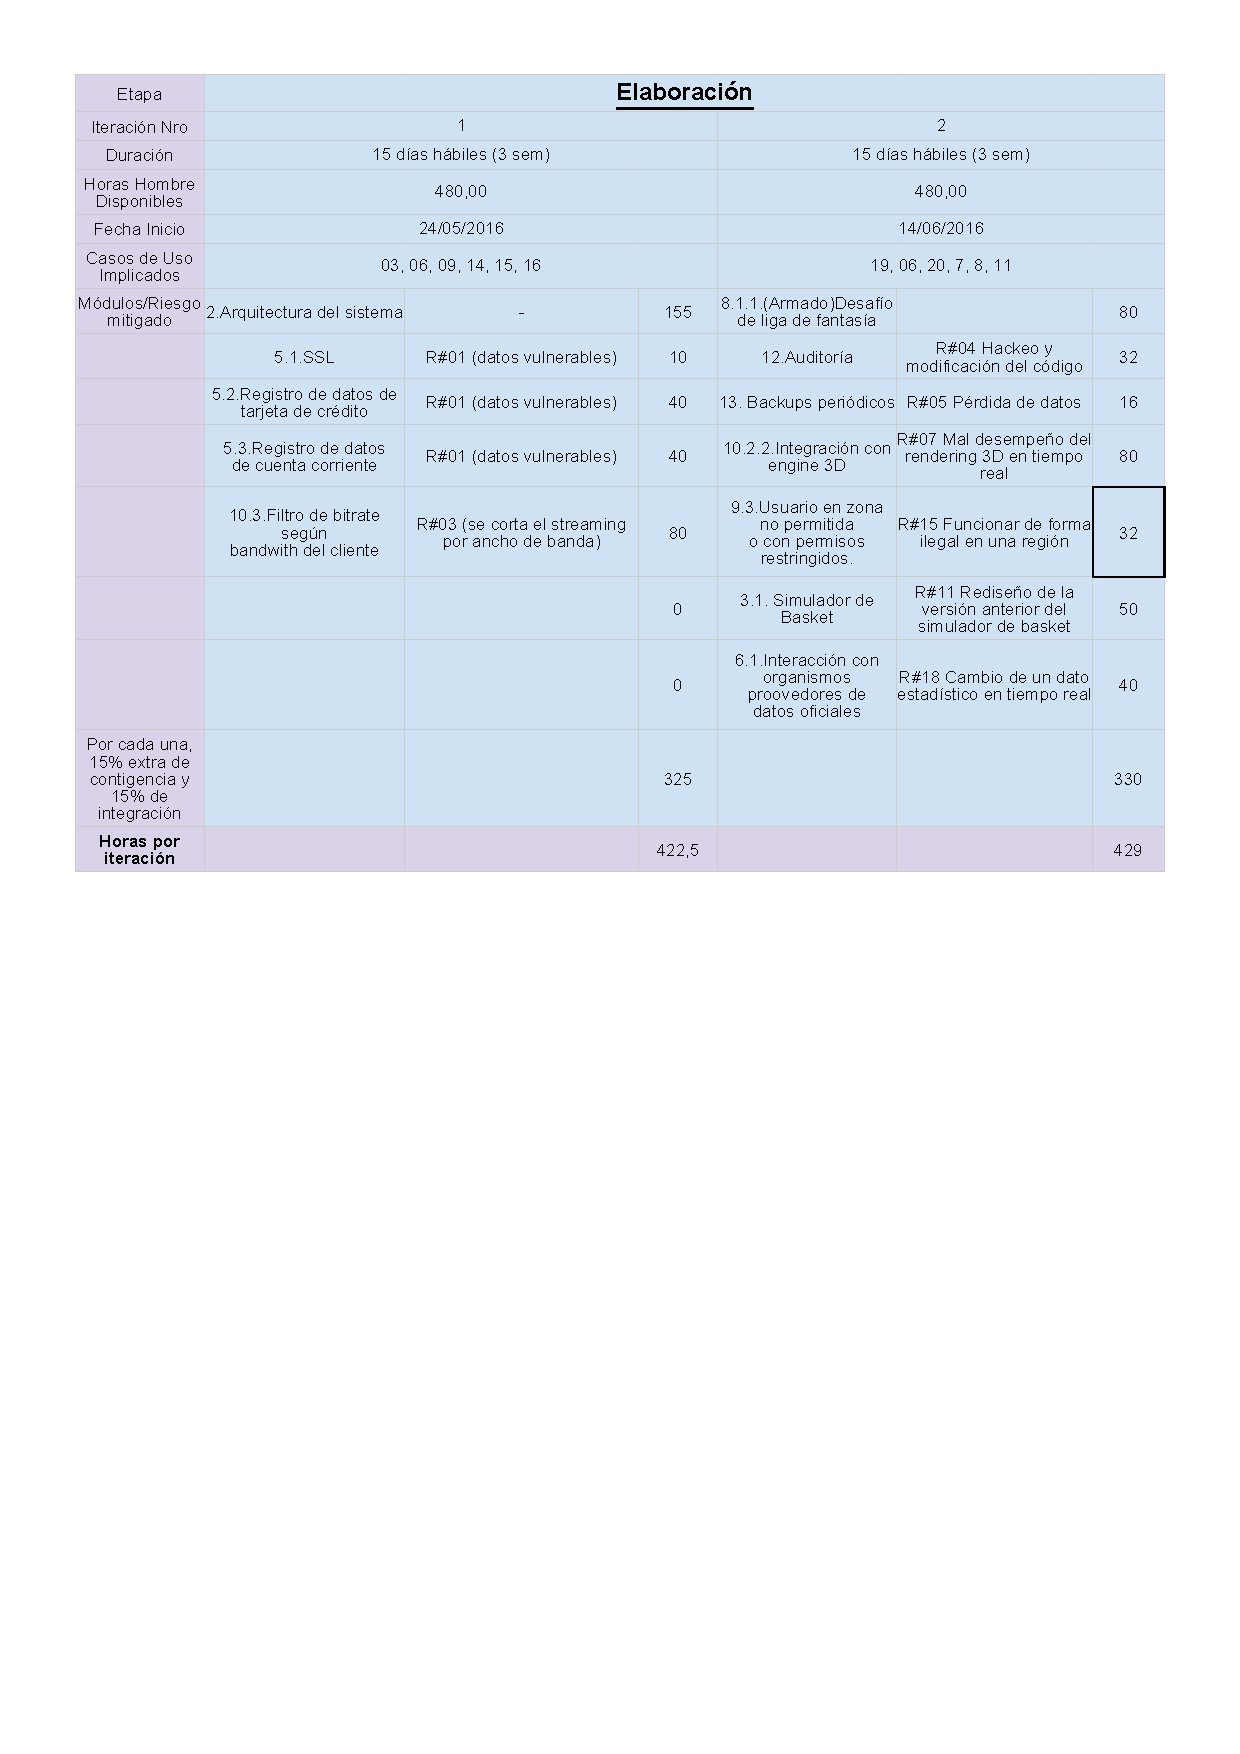
\includegraphics[scale=0.80]{imagenes/etapas-elaboracion.pdf}
   \caption{División de tareas en la etapa de elaboración}
\end{figure}

En la etapa de construcción se desarrollan los módulos y casos de uso faltantes faltantes de forma iterativa incremental. 

Finalmente en la etapa de transición se realizan tareas de mantenimiento.

\newpage
\begin{landscape}

\begin{figure}[h!]
   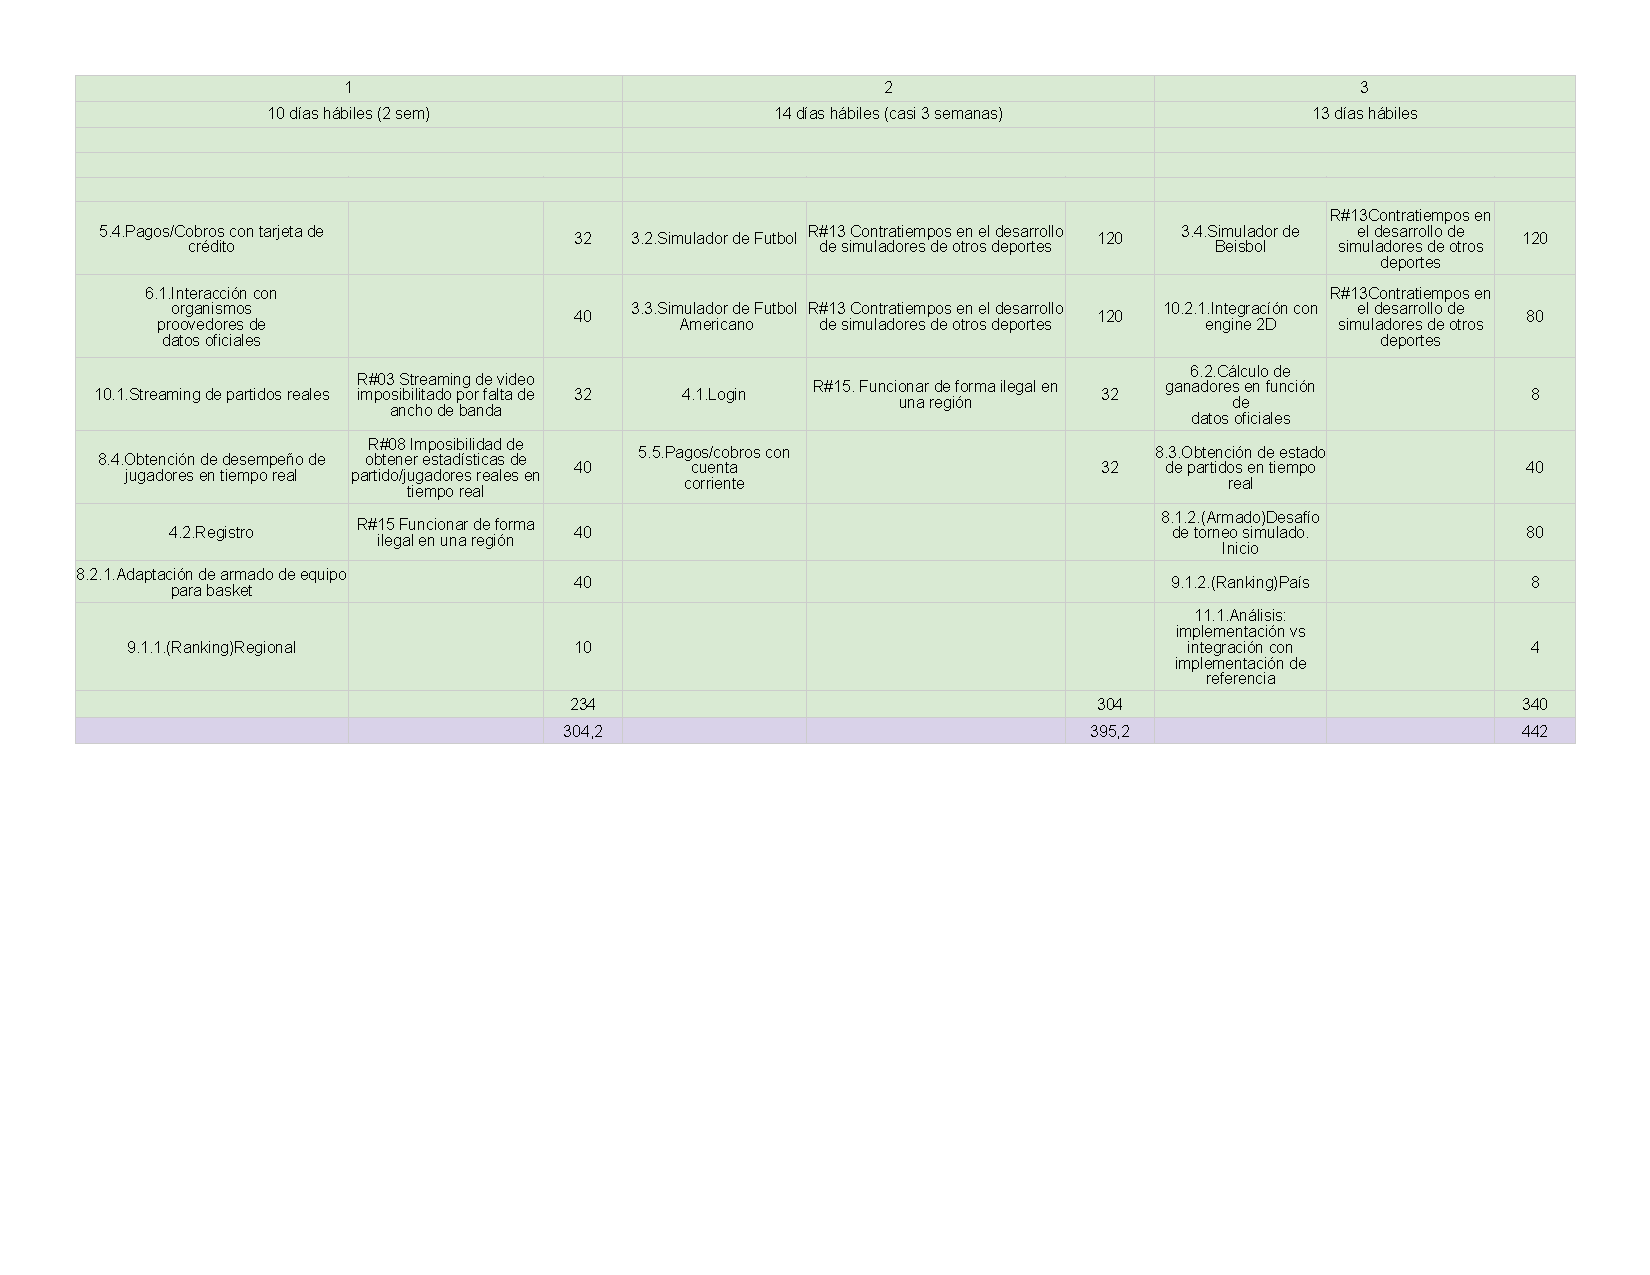
\includegraphics[scale=0.8]{imagenes/construccion123.pdf}
   \caption{División de tareas de las primeras 3 iteraciones de la etapa de 'Construcción'}
\end{figure}

\end{landscape}
\newpage

\newpage
\begin{landscape}

\begin{figure}[h!]
   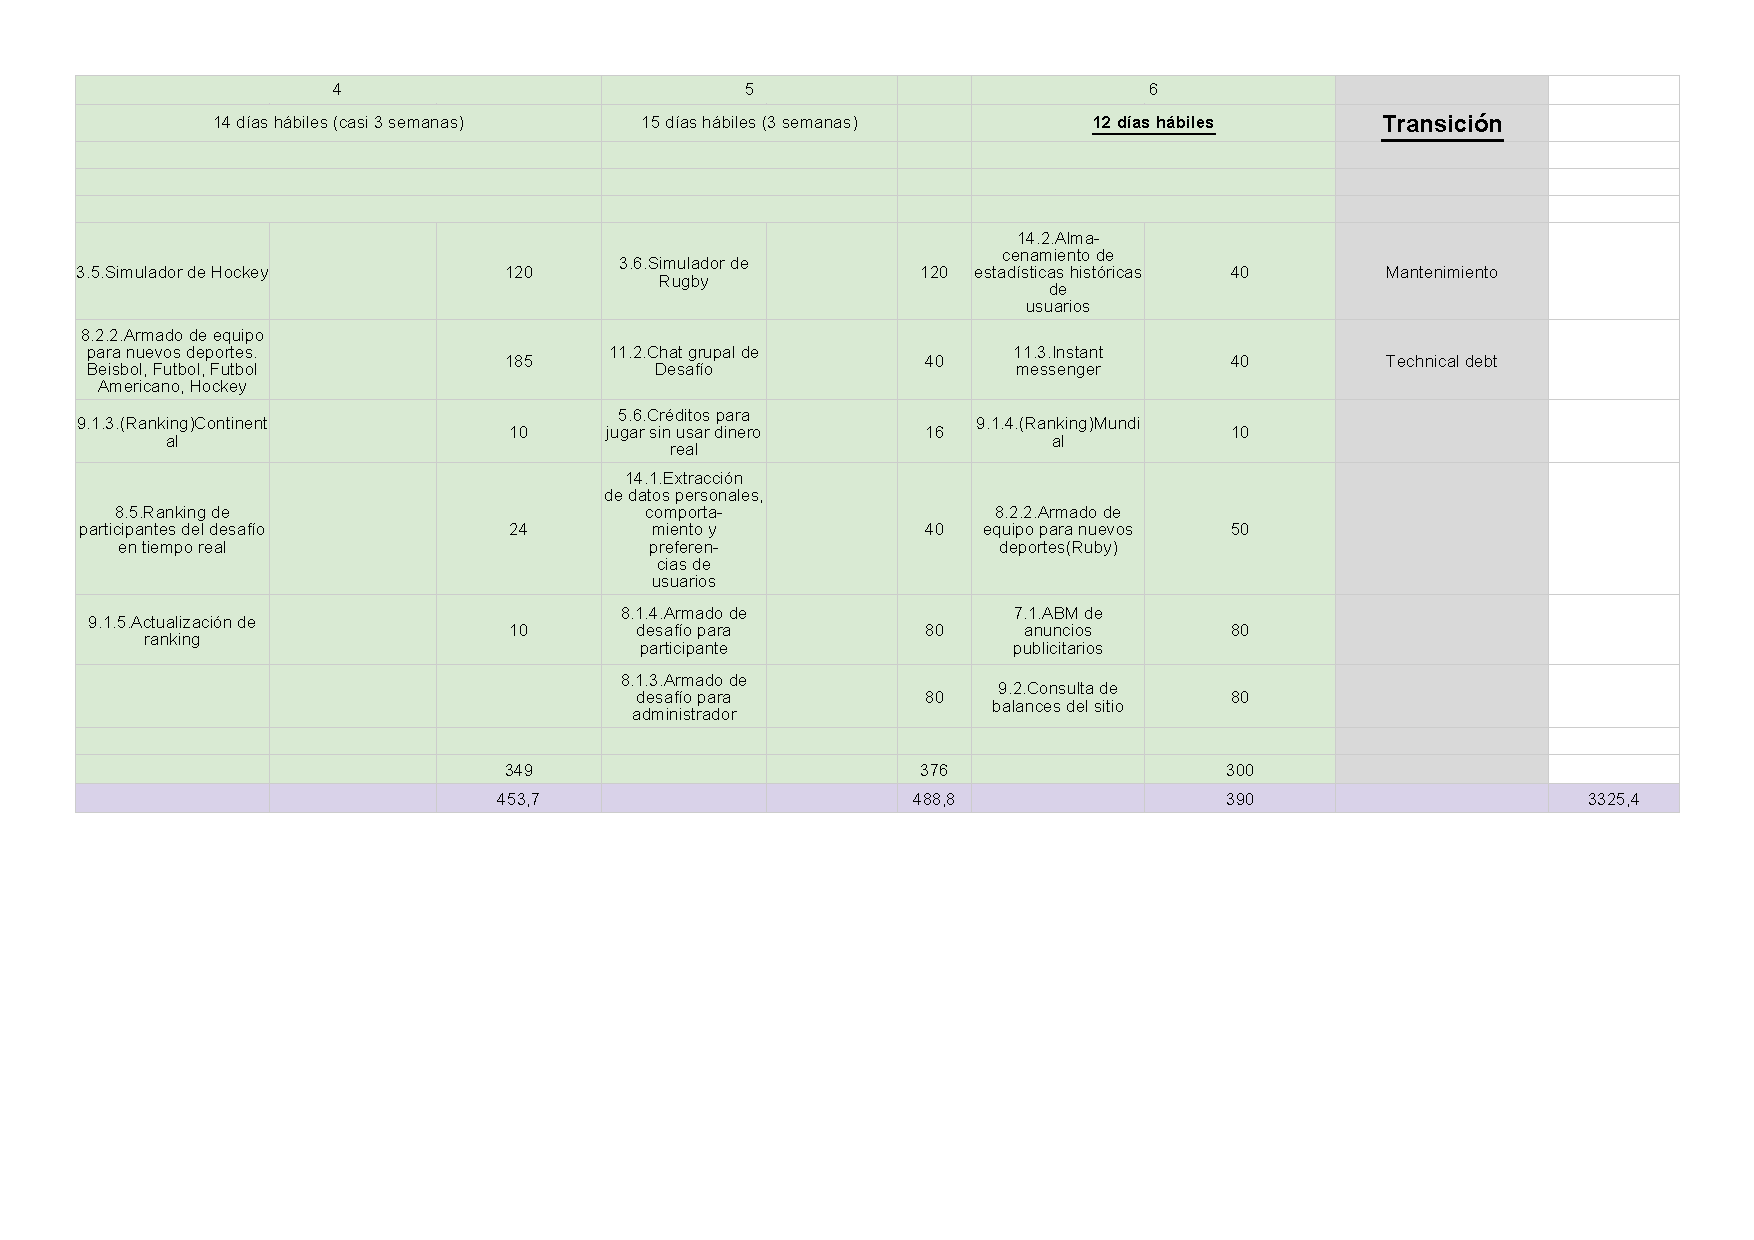
\includegraphics[scale=0.8]{imagenes/construccion-transicion.pdf}
   \caption{División de tareas de las últimas 3 iteraciones de la etapa de 'Construcción' y 'Transicion'}
\end{figure}

\end{landscape}
\newpage




% \subsection{Estimación de Módulos}
% A continuación se estima en horas hombre los módulos de nivel 1 y 2 del WBS. La estimación se basa en un grupo de trabajo de 4 recursos de 8 horas cada uno, 20 días por mes. Las horas hombre son las horas totales a consumir entre los 4 recursos sumados. Al final se realiza una sumarización de los números para estimar la duración total del proyecto.

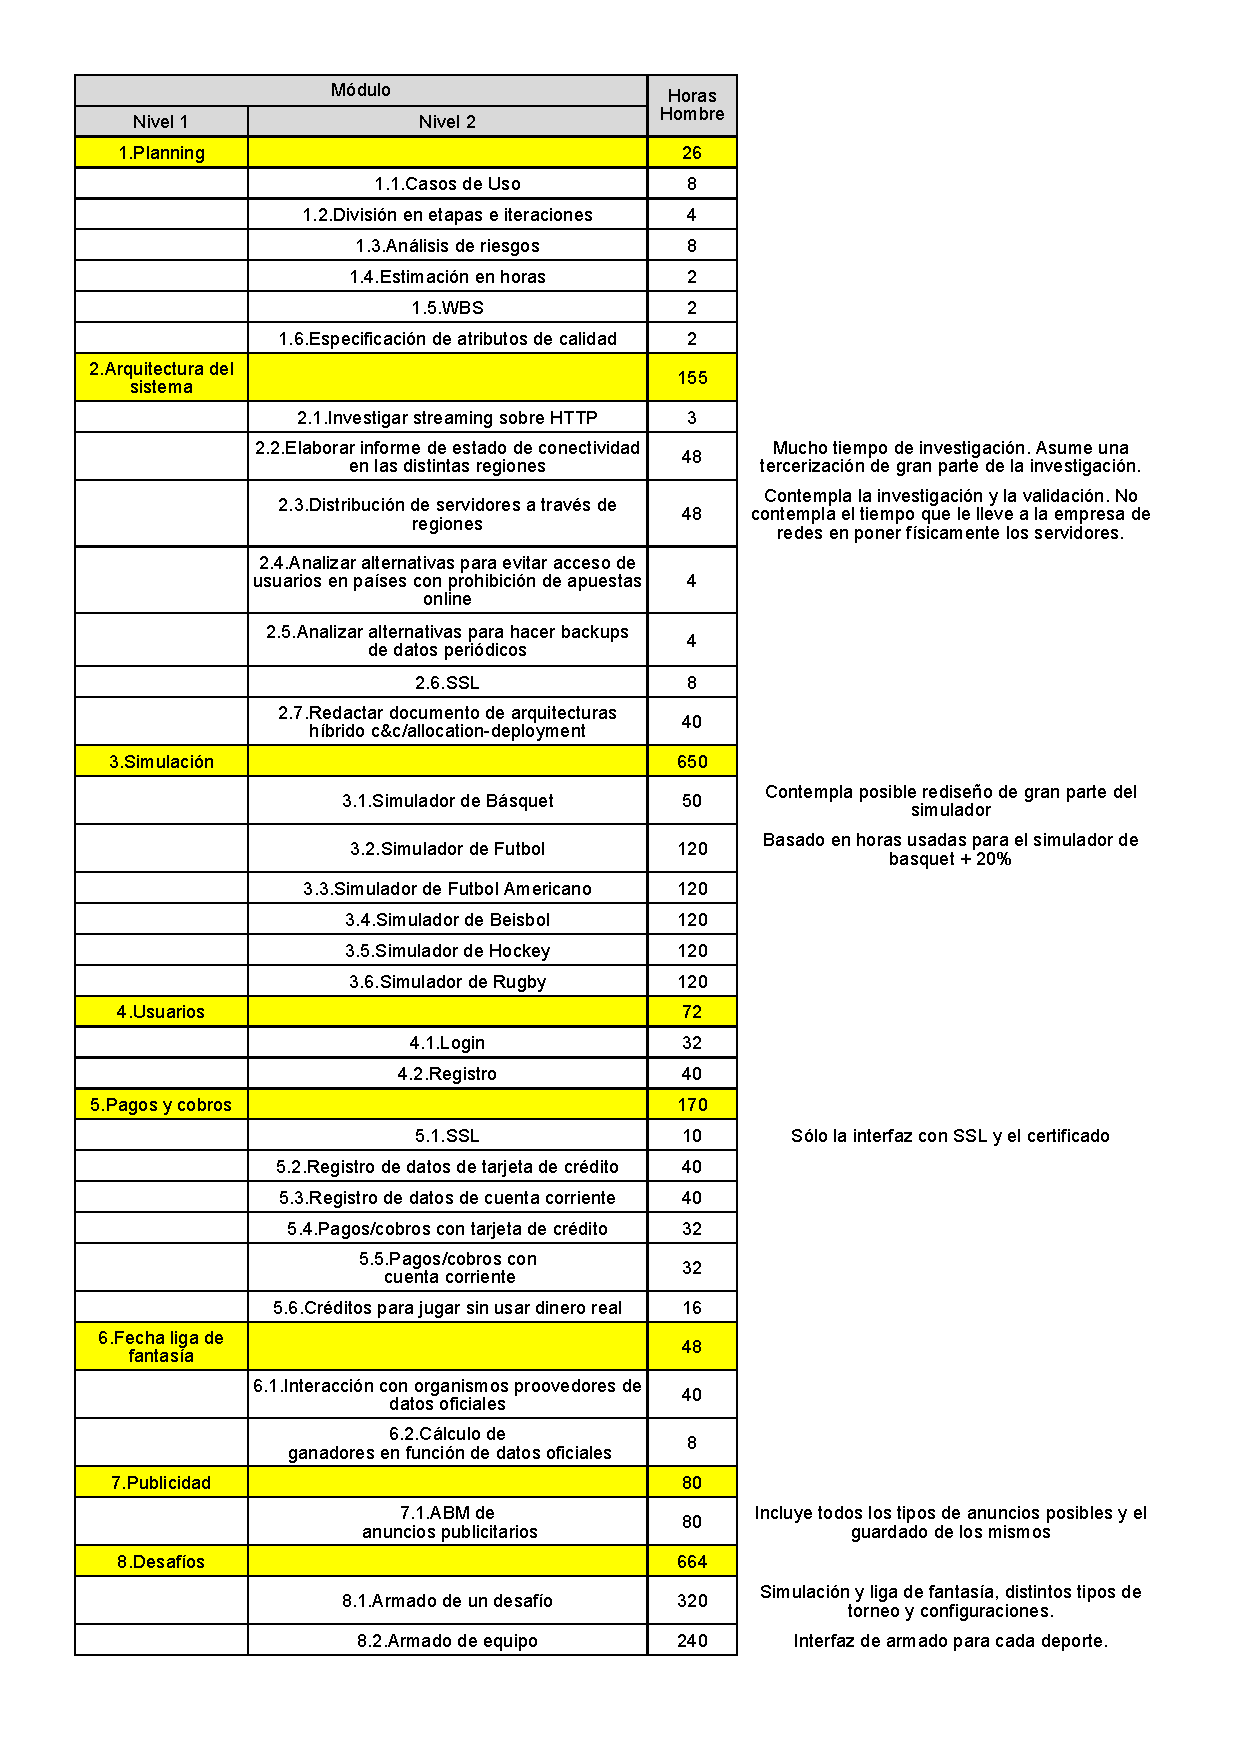
\includegraphics[width=\textwidth, page=1, clip, trim=20 0 20 30]{imagenes/estimacionModulos.pdf}

\newpage
\includegraphics[width=\textwidth, page=2, clip, trim=20 200 20 30]{imagenes/estimacionModulos.pdf}

Como puede observarse, el total estimado es bastante razonable para la magnitud del proyecto. Los tiempos podrían acelerarse si se contratara más gente y se tuviera un grupo de trabajo de 2 o 3 personas en cada módulo. Se estima que en 5 meses el proyecto debería estar funcionando, salvando las demoras que puedan causar los proveedores en responder y realizar su trabajo.
% \subsection{Division en etapas e iteraciones}
% En el proceso de elaboración se incluyen las tareas relacionadas con la arquitectura del sistema, y se genera una base ejecutable del código sobre la cual se pueda 
empezar a testear dicha arquitectura.

Al mismo tiempo se desarrollan los componentes con un rol central dentro de la arquitectura definida, y los módulos de los casos de uso con más riesgos
de alto impacto a nivel estructural, dejando cada una en una iteración diferente. La idea es construir la arquitectura de forma incremental. La opción a nivel arquitectura propuesta
en cada iteración debe ser compatible con la anterior, y al mismo tiempo solucionar el caso de uso actual.

\begin{figure}[h!]
   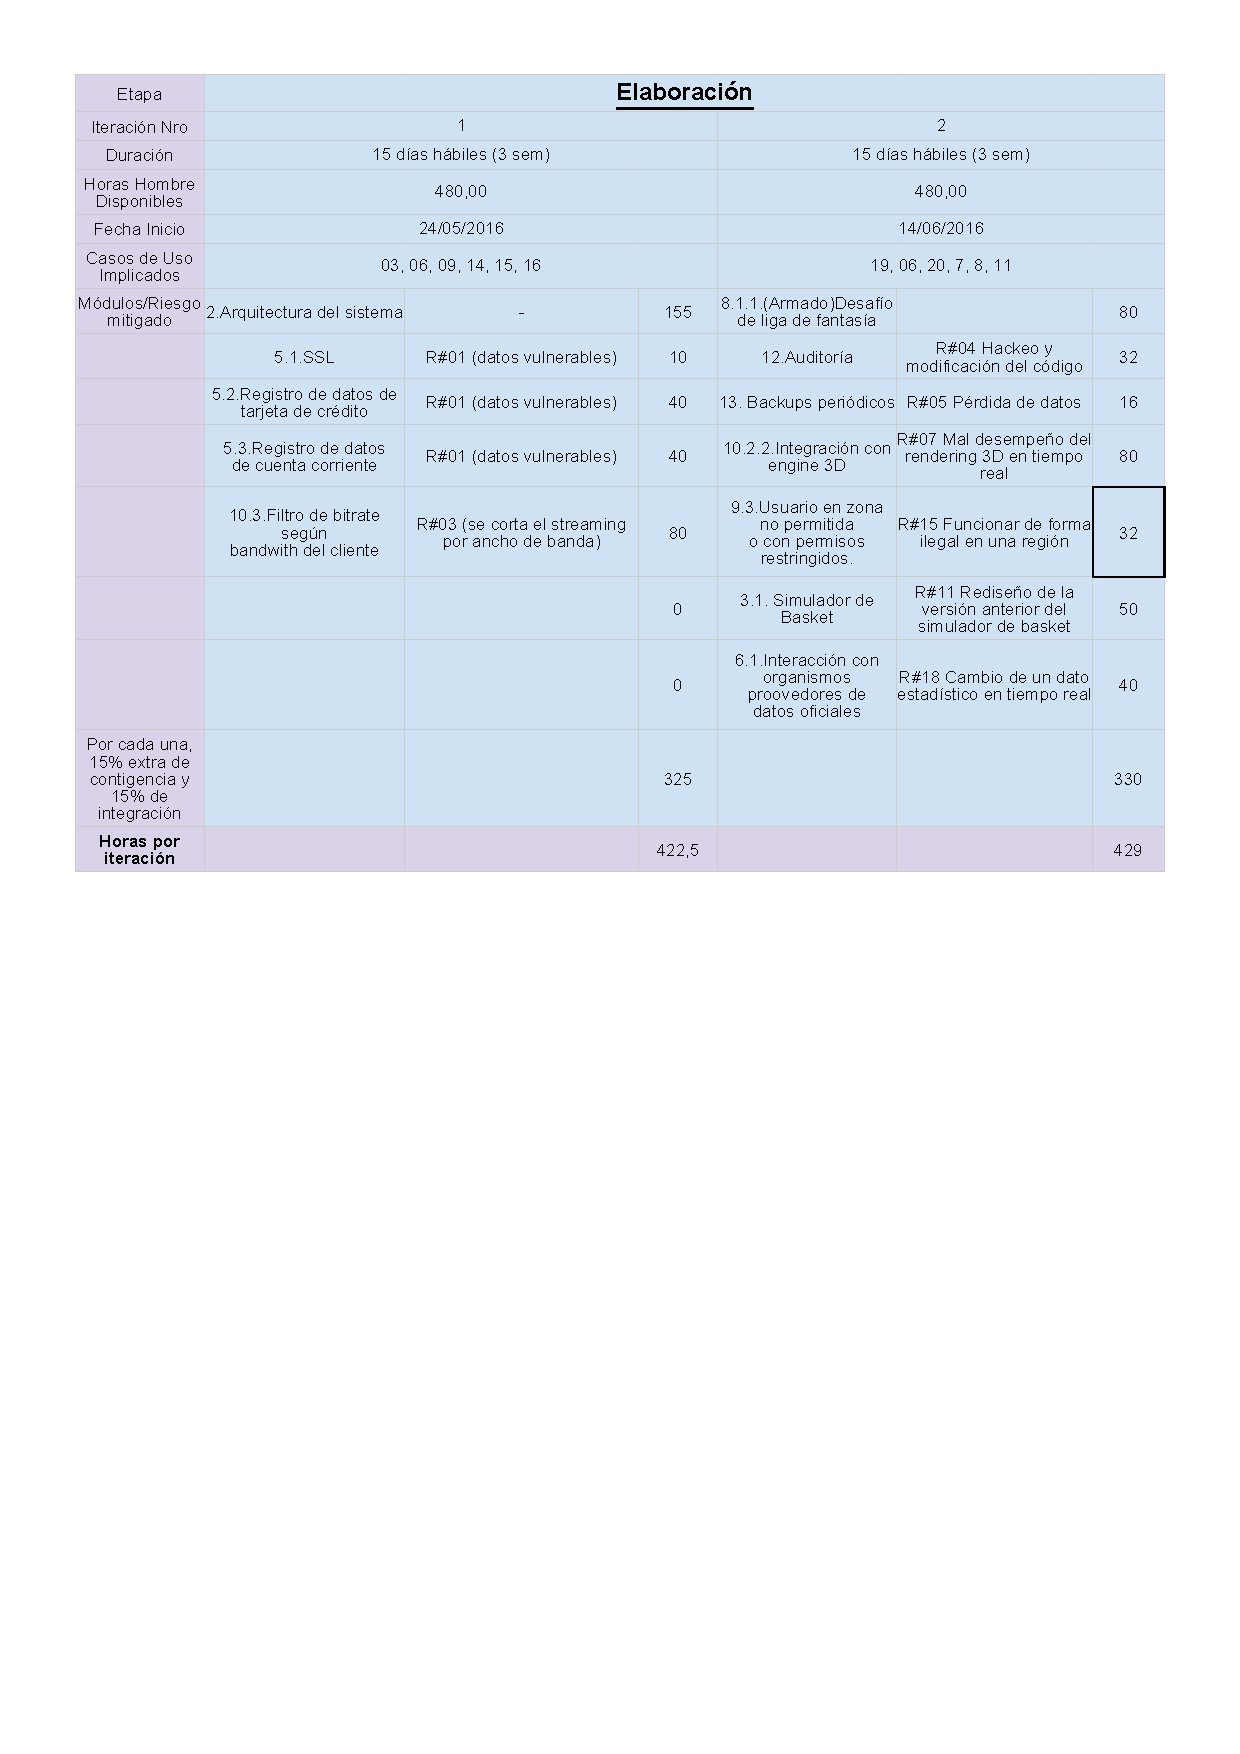
\includegraphics[scale=0.80]{imagenes/etapas-elaboracion.pdf}
   \caption{División de tareas en la etapa de elaboración}
\end{figure}

En la etapa de construcción se desarrollan los módulos y casos de uso faltantes faltantes de forma iterativa incremental. 

Finalmente en la etapa de transición se realizan tareas de mantenimiento.

\newpage
\begin{landscape}

\begin{figure}[h!]
   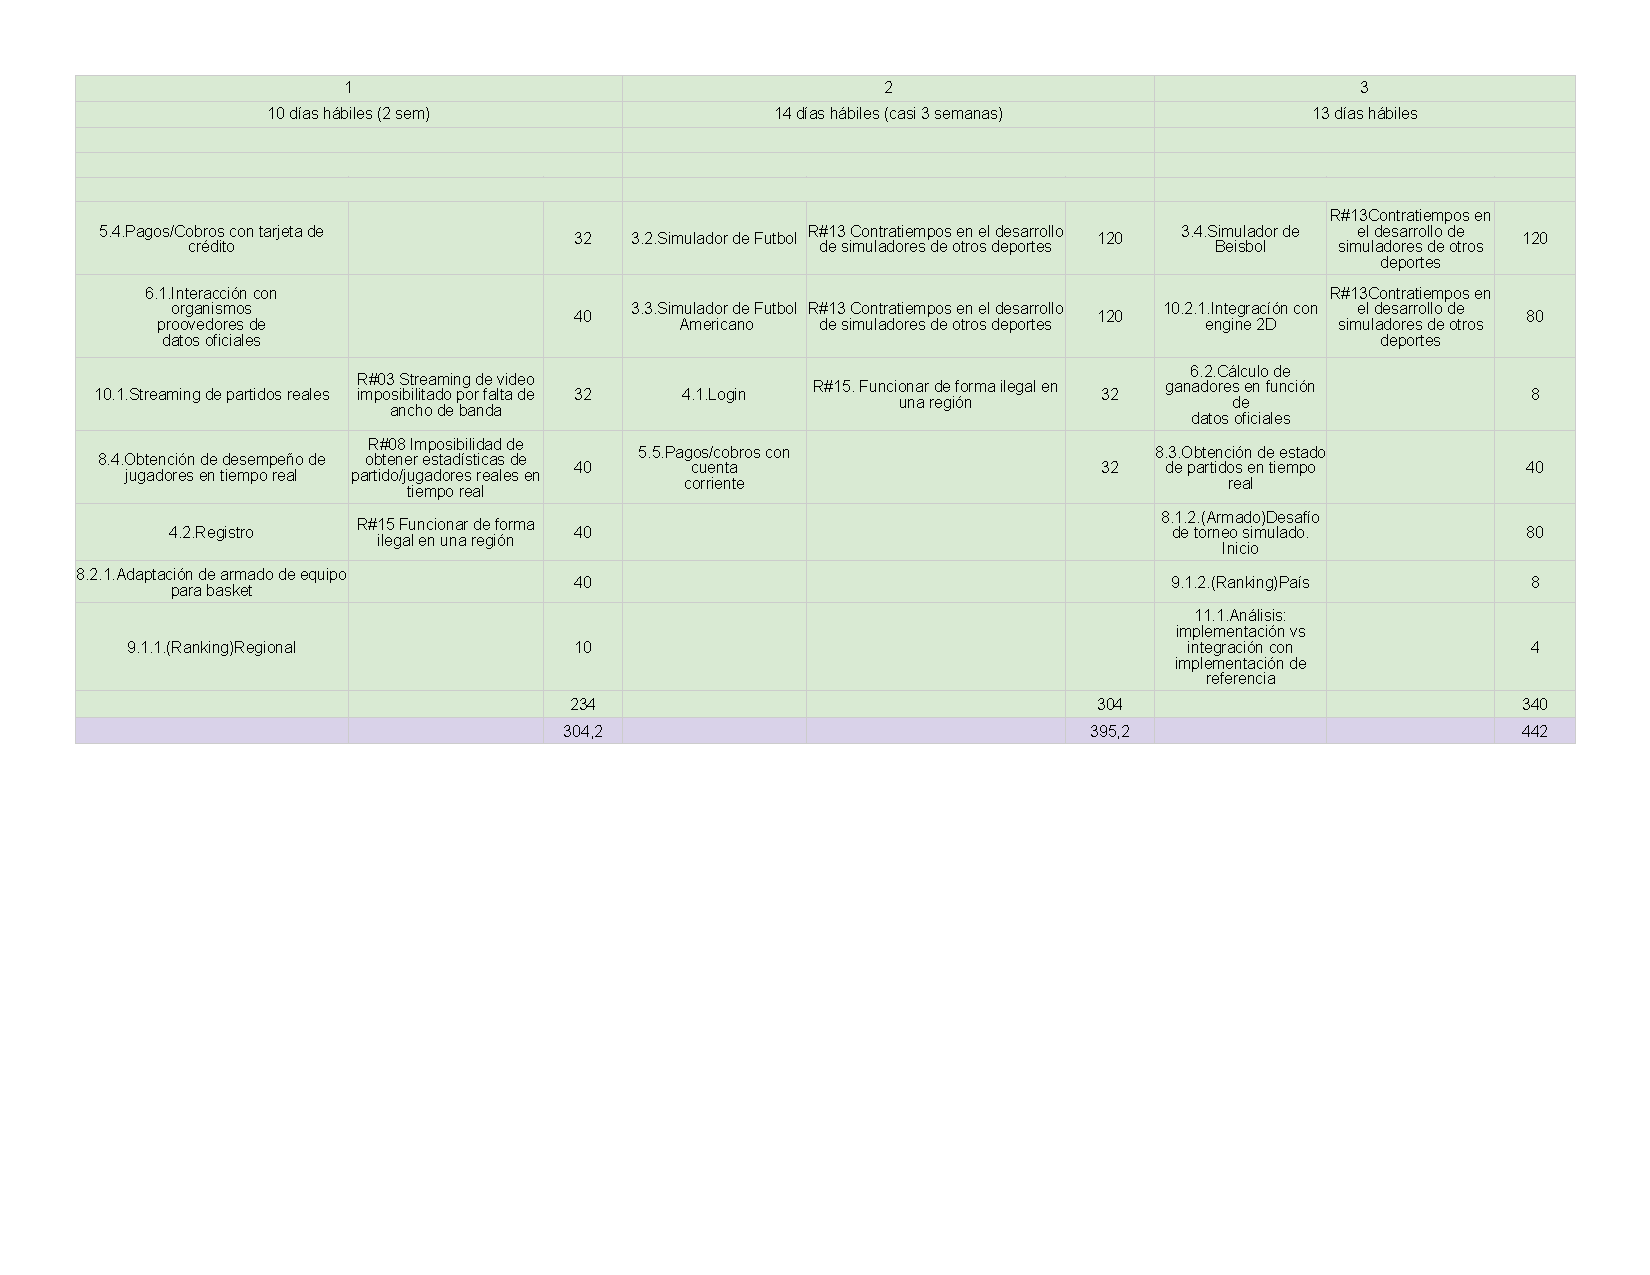
\includegraphics[scale=0.8]{imagenes/construccion123.pdf}
   \caption{División de tareas de las primeras 3 iteraciones de la etapa de 'Construcción'}
\end{figure}

\end{landscape}
\newpage

\newpage
\begin{landscape}

\begin{figure}[h!]
   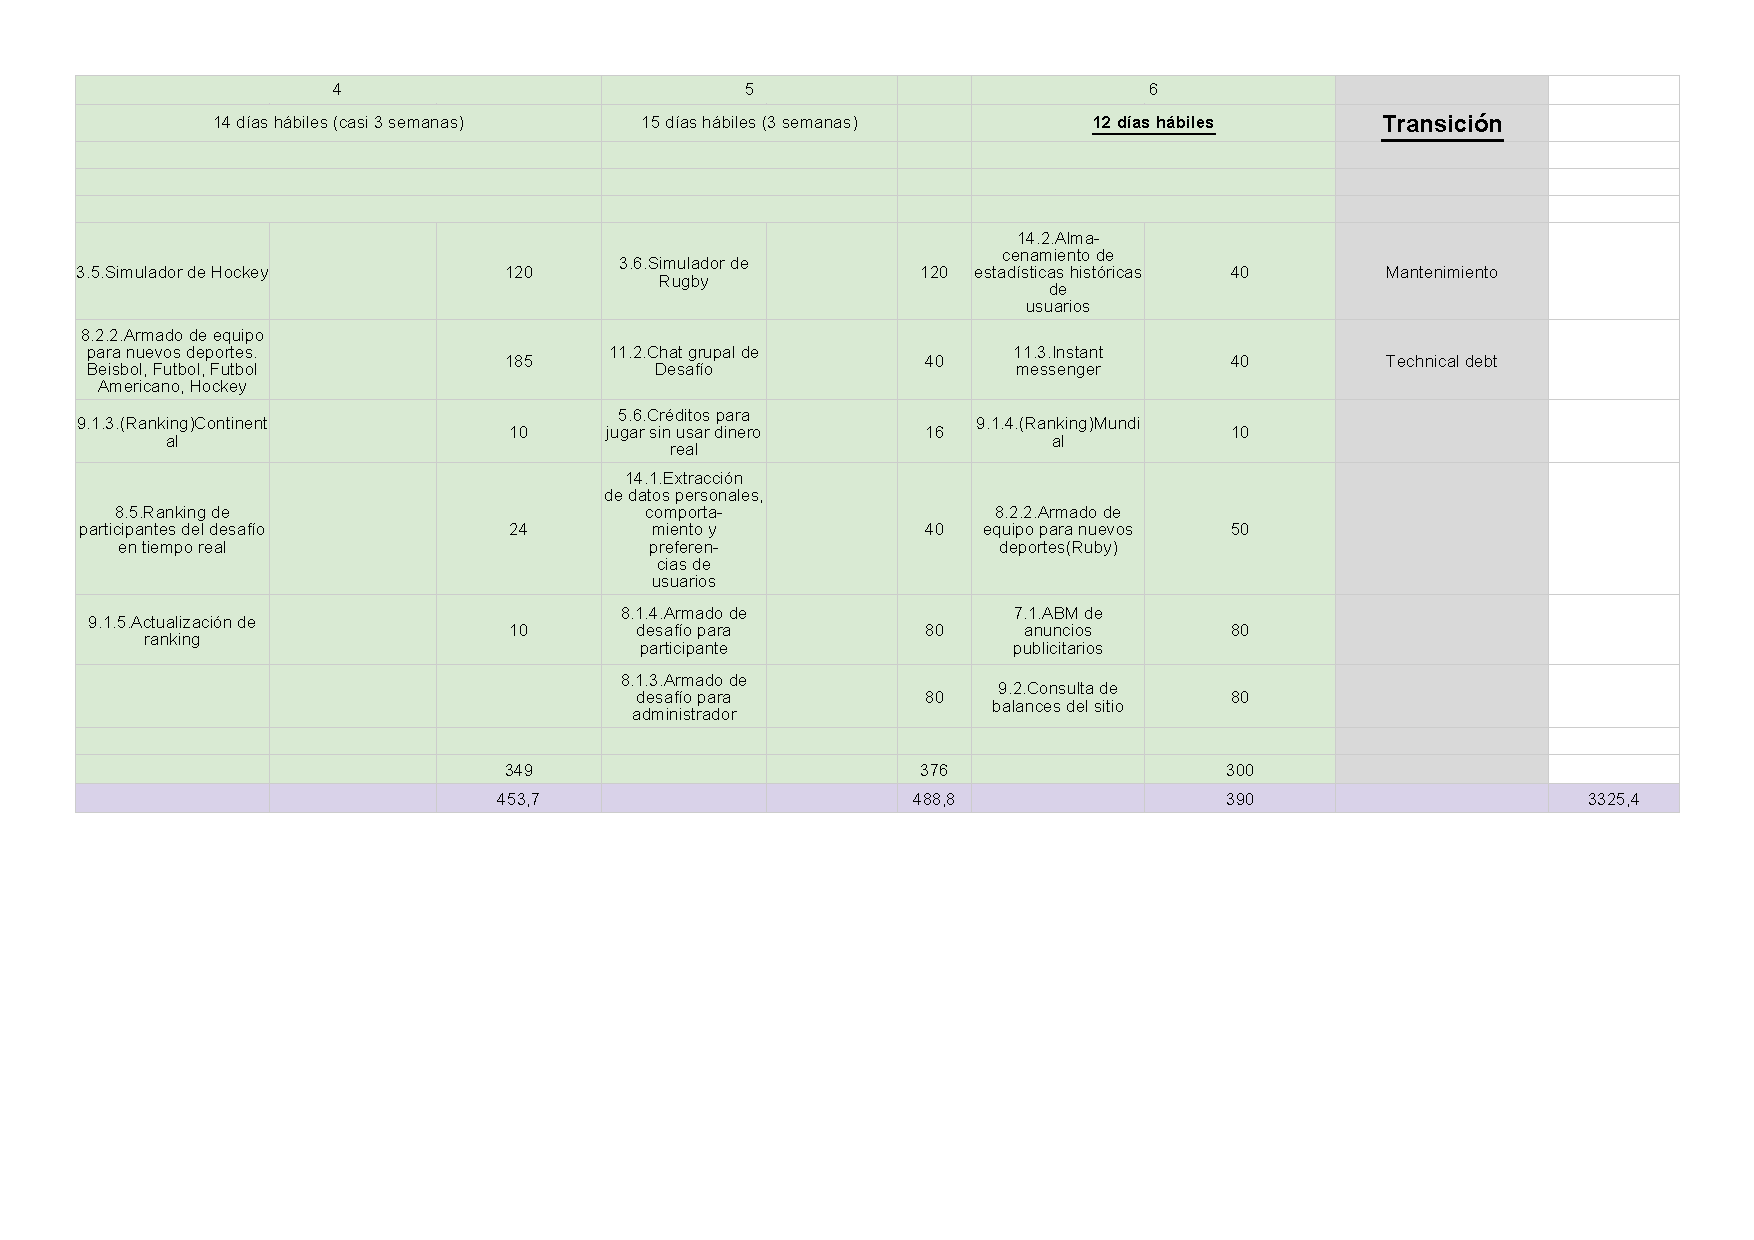
\includegraphics[scale=0.8]{imagenes/construccion-transicion.pdf}
   \caption{División de tareas de las últimas 3 iteraciones de la etapa de 'Construcción' y 'Transicion'}
\end{figure}

\end{landscape}
\newpage




\section{Primer Entrega}
No realizamos ninguna correción sobre la primer entrega, por lo que no la volvemos a presentar en esta
entrega.
\newpage
\section{Atributos de calidad}
En esta sección presentamos los escenarios de calidad que obtuvimos tras analizar los resultados del QAW.

\subsection{Atributos de disponibillidad}

\escenario
{Atributo de disponibilidad}
{El sistema debe estar andando todo el tiempo}
{Externa}
{Solicita acceso al sistema}
{Normal}
{Sistema}
{El sistema responde normalmente}
{Disponibilidad del 99,99\% (se puede caer aprox 1h en todo el año)}


~

\escenario
{Atributo de disponibilidad}
{Si falla un enlace regional, se redirige el tráfico a regiones cercanas de manera uniforme.}
{Servidor regional}
{No responde}
{Normal}
{Sistema}
{El sistema detecta la falla en el servidor regional y redirige el tráfico a las regiones más cercanas. La región entra en modo degradado. Se loguea la falla y se envía una notificación al técnico en redes}
{El servidor / enlace son reparados en menos de 24hs.}


~

\escenario
{Atributo de disponibilidad}
{Se produce una falla en una base de datos de un servidor}
{Interna}
{Falla en la base de datos de un servidor}
{Normal}
{Subsistema de almacenamiento y manejo de datos persistidos}
{El subsistema detecta y loguea la falla. El servidor originial continúa operando normalmente a través del uso de votación. La base de datos cambia a silencioso en el caso de ser la primera falla, y es reemplazada por una nueva instancia en caso de ser la segunda. Se envía una notificación al Data Base Manager.}
{Se garantiza disponibilidad a pesar de una falla en la base de datos el 99.99\% de las veces}

~

\escenario
{Atributo de disponibilidad}
{Se pierden datos de una base de datos de servidor}
{Interna}
{Pérdida de datos en una base de datos de servidor }
{Normal}
{Subsistema de almacenamiento y manejo de datos persistidos}
{El subsistema detecta y loguea la falla. El servidor recupera los datos ya que cuenta con una base redundante. La base de datos cambia a silencioso en el caso de ser la primera falla, y es reemplazada por una nueva instancia en caso de ser la segunda. Se envía una notificación al Data Base Manager.}
{Se mantienen los datos a pesar de una pérdida en una de las bases de datos el 99.99\% de las veces}

~

\escenario
{Atributo de disponibilidad}
{Se pierden los datos de todas las bases de datos de servidor}
{Interna o externa}
{Perdida de datos de todas las bases de datos de servidor}
{Normal}
{Subsistema de almacenamiento y manejo de datos persistidos}
{El subsistema detecta y loguea la falla. El servidor vuelve al último estado consistente de las últimas 4 horas, ya que realiza un backup cada esa cantidad de tiempo. Se restauran todas las bases. Se envía una notificación al Data Base Manager.}
{La probabilidad del escenario anterior es $<$ 0.00001\%. Las bases se restauran en un tiempo $< 4$ horas}

~

\escenario
{Atributo de disponibilidad}
{En cada región habrá varios servidores con una capacidad máxima de usuarios que puede atender, debido a limitaciones de hardware / conexión. Si nuevos usuarios se agregan y superan el 90\% de la capacidad, habrá que agregar un nuevo servidor y balancear la carga}
{Externa}
{Solicita acceso al sistema}
{A 1 pedido de alcanzar el límite de usuarios}
{Servidor regional}
{El servidor responde normalmente. Se incorpora un nuevo servidor a la red, y se aplica el balanceo de carga correspondiente}
{Se realiza la subdivisión de la región agregando un nuevo nodo en menos de 6 horas}

~

\escenario
{Atributo de disponibilidad}
{Enlaces congestionados durante streaming de partido real}
{Externa}
{Disminución de la capacidad de enlace durante streaming de partido real}
{Normal}
{Servidor regional}
{Se detecta el cambio de bitrate. Se realiza un downgrade de la calidad de video. El usuario continúa observando el partido de forma fluída, pero con menor calidad.}
{El streaming del video mantiene un rate constante de cuadros por segundo el 99.99\% de los casos}

~

\escenario
{Atributo de disponibilidad}
{Enlaces congestionados durante streaming de video de simulación}
{Externa}
{Disminución de la capacidad de enlace durante streaming de simulación}
{Normal}
{Servidor regional}
{Se detecta el cambio de ancho de banda del enlace. Se realiza un downgrade en el bitrate}
{El streaming de la simulación mantiene un rate constante de cuadros por segundo el 99.99\% de los casos}

~

\escenario
{Atributo de disponibilidad}
{Se caen enlaces de región durante transmisión de torneo continental o mundial}
{Externa}
{Caída de enlaces de región durante transmisión de torneo continental o mundial}
{Normal}
{Servidor regional}
{Se detecta la caída de los enlaces en la región. Se utiliza la topología de la conexión de regiones para triangular los paquetes y que lleguen a los usuarios.}
{El 99.99\% de las veces el usuario continúa viendo la transmisión del evento sin cortes abruptos, experimentando a lo sumo un cambio en la calidad del video}

\subsection{Atributos de performance}

\escenario
{Atributo de performance}
{Quiere que todo lo respectivo al manejo de dinero (depósitos y retiros de los participantes
via tarjeta de crédito o caja de ahorro) sea super seguro (no quiere papelones y que los
datos de las millones de tarjetas de los participantes aparezcan publicados en Reddit),
transparente y rápido. Que los datos queden resguardados y sólo haya que actualizarlos
esporádicamente.}
{usuario}
{depósito / retiro de dinero}
{operación normal}
{subsistema de pagos}
{el sistema realiza la operación satisfactoriamente}
{el sistema realiza la operación en menos de 15 segundos}

~

\escenario
{Atributo de performance}
{Propone un sistema de bitrate variable automático/manual de los streams de video para
que se pueda bajar la calidad de los videos en base al bandwidth detectado disponible del
usuario.}
{usuario}
{observa transmisión de partido}
{sistema degradado}
{sistema}
{se modifica calidad del video}
{se modifica la calidad del video en menos de 10 segundos}

~

\escenario
{Atributo de performance}
{Quiere que mientras sea posible se use el engine 3d de mayor calidad al 2d.}
{usuario}
{observa simulación de partido}
{sistema degradado}
{dispositivo móvil antiguo}
{se reemplaza engine 3d por 2d}
{antes de comenzar la reproducción de la simulación se reemplaza el engine 3d por 2d}


\subsection{Atributos de seguridad}

\escenario
{Atributo de seguridad}
{Atacante intenta robar datos de tarjetas de crédito o cuentas corrientes bancarias, pero el sistema lo impide}
{Atacante}
{Intenta robar datos de tarjetas de crédito o cuentas corrientes almacenados en servidores}
{Normal}
{Datos del sistema}
{Se detecta y se impide el ataque.}
{Se detecta y se impide el 99\% de los ataques.}

~

\escenario
{Atributo de seguridad}
{Atacante roba datos de tarjetas de crédito o cuentas corrientes bancarias, pero no puede descifrarlos}
{Atacante}
{Roba datos de tarjetas de crédito o cuentas corrientes almacenados en servidores}
{Normal}
{Datos del sistema}
{Se guardan los datos en un formato imposible de leer.}
{Toma más de 1000 años descifrar los datos.}

~

\escenario
{Atributo de seguridad}
{Atacante intercepta comunicación del sistema con el usuario.}
{Atacante}
{Interviene pasivamente una comunicación entre el usuario y el sistema}
{Normal}
{Comunicación del sistema}
{La comunicación está protegida por SSL, con lo cual el contenido de los paquetes es imposible de leer}
{Toma más de 1000 años descifrar los datos interceptados}


~

\escenario
{Atributo de seguridad}
{Atacante se hace pasar por el sistema para robarle datos al usuario.}
{Externa}
{Interviene activamente una comunicación entre el usuario y el sistema, tomando el rol del sistema}
{Normal}
{Comunicación del sistema}
{El sistema utiliza un mecanismo de autenticación del servidor mediante certificados y clave asimétrica. El browser alerta al usuario de que se han vulnerado los certificados SSL. Los paquetes obtenidos por el atacante están encriptados, por lo cual su contenido no puede determinarse}
{Los usuarios advertidos acerca del posible riesgo comienzan una nueva sesión segura el 99.99\% de las veces. En el caso de que el usuario envíe datos sin darse cuenta, toma más de 1000 años descifrar los datos interceptados}

~

\escenario
{Atributo de seguridad}
{Atacante modifica mensajes enviados entre el sistema y el usuario para forzar al sistema a realizar acciones no solicitadas por el usuario.}
{Externa}
{Interviene activamente una comunicación entre el usuario y el sistema, modificando mensajes capturados en el canal de comunicación}
{Normal}
{Comunicación del sistema}
{El sistema utiliza un mecanismo de verificación de integridad de los mensajes recibidos, tanto del lado del cliente como del servidor. El mecanismo de integridad viaja encriptado para evitar que sea modificado.}
{Toma más de 1000 años encontrar un mensaje que estando modificado tenga sentido y verifique la integridad.}

~

\escenario
{Atributo de seguridad}
{Un usuario logueado logra vulnerar el subsistema de pagos y cobros.}
{Usuario identificado}
{Vulnera el subsistema de pagos y cobros y genera movimientos de dinero a su favor}
{Normal}
{Subsistema de pagos y cobros}
{El sistema tiene un audit trail con el registro de todas las acciones realizadas por todos los usuarios logueados y revierte las operaciones realizadas por el usuario.}
{El 99.99\% de las veces el log tiene todos los datos necesarios para revertir las operaciones del usuario.}

~

\escenario
{Atributo de seguridad}
{Usuario no autorizado desea hacer uso de los datos recolectados por minería}
{Usuario sin privilegios de administrador}
{Intento de acceso a datos recolectados por minería}
{Normal}
{Sistema}
{El sistema loguea el intento de acceso. El sistema valida los permisos del usuario en el sistema y posteriormente niega el acceso}
{Los usuarios no autorizados no logran acceder a los datos el 99.99999\% de los casos}

~

\escenario
{Atributo de seguridad}
{Auditor verifica que el código de la simulación y cálculo de resultados de desafíos no se haya modificado}
{Auditor}
{Solicitud de hashes de auditoría para módulos de simulación y cálculo de resultados de desafíos}
{Normal}
{Sistema}
{Se otorgan los hashes correspondientes a ambos módulos}
{La coincidencia de los hashes obtenidos con los conservados con el auditor garantizan que el código no ha cambiado el 99.9999\% de los casos (muy baja probabilidad de colisiones en la función de hash)}

~

\escenario
{Atributo de seguridad}
{Usuario culpa al sistema de que no se le ha asignado el premio de un desafío en el que ha participado y ganado, pero no figura su lista de desafíos}
{Usuario}
{Acusación de premio no otorgado}
{Normal}
{Sistema}
{Se le muestra en base al audit trail del sistema el listado de todas las inscripciones a desafíos que realizó, quedando en evidencia que el usuario no se ha inscripto en dicho desafío}
{El audit trail mantiene una relación 1 a 1 con las operaciones del usuario en un 99.99\% respecto a las acciones del usuario del sistema. Es decir, no hay acciones que no estén logueadas y en el log aparecen únicamente acciones realizadas por dicho usuario}

~

\escenario
{Atributo de seguridad}
{Resolvedor de desafío de liga de fantasía obtiene un dato erróneo de una jugada provisto por el sistema externo que brinda resultados en real-time}
{Externa}
{Dato erróneo del sistema proveedor}
{Normal}
{Sistema}
{La resolución de una jugada en el minuto a minuto de un desafío de liga de fantasía es obtenida a partir de una votación, por lo que el resultado correcto es calculado}
{El proceso de votación obtiene el resultado correcto el 99.99\% de las veces}

\subsection{Atributos de modificabilidad}

\escenario
{Atributo de modificabilidad}
{Quiere ver estadísticas acerca del comportamiento de los participantes de todas las
temporadas (los más ganadores/perdedores en desafíos/dinero, los mejores/peores
equipos formado por participantes de diferentes caps, valores de caps de participantes,
rankings de regiones más ganadoras en desafíos/dinero, el modo de desafío más utilizado
por los participantes, etc...). Lo que está en paréntesis son sólo ejemplos. Quiere que la
mayor cantidad de datos que el sitio maneja pueda ser fácilmente minada por datos. Y
que esos datos pueda estar a cargo de administradores expertos para luego crear
desafíos acordes o otorgar créditos a participantes que califiquen.}
{administrador}
{agregar estadísticas acerca del comportamiento de los participantes}
{tiempo de ejecución}
{sistema}
{se agrega las nuevas estadísticas}
{se agregan las nuevas estadísticas en menos de una hora sin reiniciar el sistema}

~

\escenario
{Atributo de portabilidad}
{Debe de poder correr en la mayor cantidad de plataformas posibles, incluyendo móviles.}
{desarrollador}
{adaptar interfaz a una nueva plataforma}
{tiempo de diseño}
{interfaz de usuario}
{se adapta la interfaz a la nueva plataforma}
{se adaptan los cambios en menos de 50hs}

~

\escenario
{Atributo de modificabilidad}
{Quiere una interfaz similar al representante de empresas con derechos de televisación (Maxi) para controlar publicidades en las simulaciones y el sitio en general.}
{administrador}
{modificar publicidad}
{tiempo de ejecución}
{interfaz para el manejo de publicidades}
{se hace modificación de las publicidades}
{se muestran las nuevas publicidades en menos de 20 segundos}

~

\escenario
{Atributo de modificabilidad}
{Plantea necesidad de regionalizar la plataforma, debido a lo limitado y la mala calidad del
hardware/servidores disponibles para la plataforma en las regiones iniciales, sobre todo
teniendo en cuenta que los streams de video pasan por “dentro” del sistema. No se está
hablando de tercerizar el servicio a sitios como Vimeo o Youtube, sino que el tráfico pase
de alguna manera por los servidores del sitio. Los enlaces físicos/hardware subyacente
implica una cantidad de usuarios limitada / máxima por servidor}
{Interna}
{Incorporación una nueva región al sistema}
{normal}
{sistema}
{se incorpora una nueva región}
{el setup de la configuración se hace en menos de 5 horas}

~

\escenario
{Atributo de modificabilidad}
{También se quiere aumentar el caudal de redes sociales que se utilizan para “afectar” las estadísticas (no solo Twitter, sino incorporar Facebook,Google+, etc.)}
{desarrollador}
{incorporar una nueva red social al sistema}
{tiempo de diseño}
{sistema}
{se incorpora la nueva red social}
{se emplean menos de 40 hs}

~

\escenario
{Atributo de modificabilidad}
{Quiere que el énfasis se de en mejorar el módulo de simulación, para que sea lo más real
posible. Tiene contacto con asociaciones de jugadores e incluso jugadores, técnicos y
periodistas deportivos de diferentes deportes, para ayudar a mejorar el motor de
reglas/simulación. También tiene contacto con empresas de redes sociales/sentiment
analysis, para ayudar a interfacear con las mismas, y mejorar el módulo de
menciones/popularidad de los jugadores. El espíritu es que toda la simulación pueda irse
mejorando poco a poco hasta que represente lo mejor posible la realidad sin que sea un
dolor de cabeza introducir cambios.}
{sponsor, stakeholder}
{agregar nuevas reglas/acciones al motor de simulación}
{tiempo de diseño}
{motor de simulación}
{reglas/acciones nuevas agregadas sin efectos secundarios}
{se invierten menos de 10hs hombre}


\subsection{Atributos de usabilidad}

\escenario
{Atributo de usabilidad}
{Quiere poder que él y sus administradores de confianza puedan ver un dashboard en
tiempo real del estado de cuenta del sitio de cada una de las regiones y niveles (incluye locales, continentales, global, etc...) y de cualquier grupo de participantes.}
{administrador}
{ver estado de cuenta del sitio}
{tiempo de ejecución}
{sistema}
{el sistema provee un dashboard con el estado de cuenta del sitio de cada una de las regiones}
{el administrador es capaz de administrar / comprender la información suministrada en menos de 5 minutos}

~

\escenario
{Atributo de usabilidad}
{Aunque no es su responsabilidad, le interesa que la interfaz gráfica de usuarios tenga la
calidad de un “juego”, sobre toda al momento de ver a los jugadores, las jugadas de los
técnicos, colocar el nombre y logo del equipo del participante, etc... con animaciones y
efectos especiales con aceleración gráfica (blurs, iluminación dinámica, depth of field, etc).}
{usuario}
{el usuario desea administrar su equipo}
{operación normal}
{Interfaz web / Móvil}
{se muestra una interfaz gráfica llena de animaciones en donde el usuario puede administrar su equipo }
{el test de usabilidad supera el 95\% de satisfacción}

~

\escenario
{Atributo de usabilidad}
{Usabilidad del subsistema controlador de publicidades en las simulaciones y en el sitio}
{Usuario administrador de publicidades}
{Desea minimizar el impacto de sus errores al configurar publicidades}
{Runtime}
{Sistema}
{Se provee un botón de cancelación para volver a la configuración anterior}
{Los cambios realizados se vuelven atrás y las publicidades no cambian.}

~

\escenario
{Atributo de usabilidad}
{Usabilidad del subsistema controlador de publicidades en las simulaciones y en el sitio}
{Usuario administrador de publicidades}
{Desea estar seguro de dónde se muestra en el sistema la publicidad que está modificando}
{Runtime}
{Sistema}
{Se provee una previsualización de cada publicidad, ubicada en el entorno gráfico que corresponde, acompañada de un texto descriptivo.}
{Durante 1 hora se le enseña a dos personas a usar la interfaz de ABM de publicidades y luego se les solicita hacer cambios en todas las publicidades. Modificarán correctamente al menos el 80\%.}

~

\escenario
{Atributo de usabilidad}
{Usabilidad del subsistema controlador de publicidades en las simulaciones y en el sitio}
{Usuario administrador de publicidades}
{Desea insertar la misma publicidad en muchos lugares del sistema de forma eficiente}
{Runtime}
{Sistema}
{Se provee una funcionalidad especial para cargar una publicidad eligiendo múltiples sitios.}
{Toma a lo sumo 3 clicks adicionales cargar una publicidad en muchos sitios que cargarla en un único sitio (además de todos los clicks necesarios para seleccionar los distintos sitios) (suponiendo que no se cometen errores en la selección de sitios).}

~

\escenario
{Atributo de usabilidad}
{Usabilidad del subsistema de pagos y cobros}
{Usuario}
{Desea estar tranquilo de que ingresar en el sistema su número de tarjeta de crédito o cuenta corriente es seguro.}
{Runtime}
{Sistema}
{Se muestran los nombres de las autoridades que auditaron la seguridad del sistema y los documentos que lo prueban.}
{En menos de 5 minutos el usuario se anima a ingresar sus datos.	}


% \escenario
% {Atributo de auditabilidad}
% {}
% {administrador}
% {buscar operaciones hechas con tarjeta de crédito}
% {operación normal}
% {sistema}
% {se muestra la operación buscada}
% {cada vez que se realiza una operación con tarjeta de crédito se guarda quién la hizo, en qué momento, en qué ip y qué monto se acreditó / retiro}














































\section{Arquitectura}
En esta sección presentamos la arquitectura que proponemos para cumplir con los atributos de calidad
ya planteados.

\subsection{Diagrama de nivel 0}
\begin{figure}[H]
  \centering
  \includegraphics[width=\textwidth]{imagenes/Nivel0.png}
  \caption{Diagrama de Arquitectura de nivel 0.}
\end{figure}
\newpage

\subsection{Diagrama de nivel 1}
\begin{figure}[H]
  \centering
  \includegraphics[width=\textwidth]{imagenes/Nivel1.png}
  \caption{Diagrama de Arquitectura de nivel 1.}
\end{figure}

El sistema se compone de N de estas instancias. Cada una representa el software que corre en un servidor. N representa la cantidad de regiones (mínima unidad geográfica) en donde corre el sistema. Cada instancia está deployada en un servidor independiente, ubicado en dicha región. Cada uno de estos servidores tiene una réplica que corre en modo shadow por si el servidor primario falla.
El sistema se compone también del conjunto de componentes que corre en los dispositivos de los usuarios.

Cada servidor almacena datos locales a su región. Las estadísticas que almacena, la información de desafíos, la información de sus usuarios son en su gran mayoría regionales, con la excepción
de que dicho servidor esté siendo utilizando para algún desafío como nodo intermedio en el árbol de jerarquía de desafíos extra-regionales. (Ver documento jeraraquía global). En ese caso,
almacena y propaga los datos del desafío que está simulando.

La comunicación entre el cliente y el servidor se realiza de 4 formas diferentes: Streaming de partido real, obtención de datos para rendering de simulación, realizar una compra de fichas
para apostar o extracción de dinero y finalmente pedidos de consulta web comunes como ser: registración, login, consulta de ranking, creación de equipo, participación de desafío, etc. Llamamos
'pedido general' a esta última categoría. Cada una de estas 4 formas de comunicación utiliza un conector distinto ya que necesitan satisfacer diferentes requerimientos.
Estos conectores tienen un estilo call-return para poner énfasis en que la comunicación es sincrónica: Un usuario hace un pedido de streaming. A partir de ese momento se inicia una
sesión entre el servidor y el usuario para mandar un flujo de datos a través del canal de comunicación que dura hasta que finaliza la conexión.

El subsistema de desafíos maneja tanto las simulaciones como las ligas de fantasía.

'Currification' tiene un acuerdo con las empresas televisivas proveedoras de transmisiones, mediante la cual permite crear enlaces para satisfacer los pedidos de los usuarios para ver
partidos televisados. El manejador de pedidos recibe los datos de cada transimisión a través de un pipe, y resuelve a través de un mapping sesiones de usuarios vs transmisiones para
saber qué transmisiones debe enviarle a cada usuario. Una situación análoga sucede con las simulaciones.

Los stakeholders pueden agregar publicidades a través de una interfaz gráfica intuitiva y simple. Esta les permite decidir en qué lugar mostrarán cada publicidad: UI de la web,
rendering de simulaciones o streaming de partidos. Por este motivo, el subsistema de publicidad rutea las nuevas publicidades a los subsistemas correspondientes.

Los controles de auditoría se hacen sobre los subsistemas de pagos y cobros (para corroborar que no haya movimientos irregulares de dinero), y sobre el subsistema de simulación de
desafíos, verificando que el hash del código de simulación no haya sido modificado.

La autenticación y restricción al sitio por parte de los usuarios se realiza a partir de reglas: Algunas direcciones de IP están restringidas. Correspondientes a aquellas zonas en donde
están prohibidas las apuestas web. Por otro lado, cuando un usuario asocia una tarjeta a su cuenta el sistema verifica que la tarjeta sea local a la región a la cual se encuentra.
Finalmente, cuando un usuario quiere realizar una compra utilizando una tarjeta, esta última debe coincidir con aquella que ha sido registrada previamente.


\newpage

\subsection{Jerarquia Virtual}
\begin{figure}[H]
  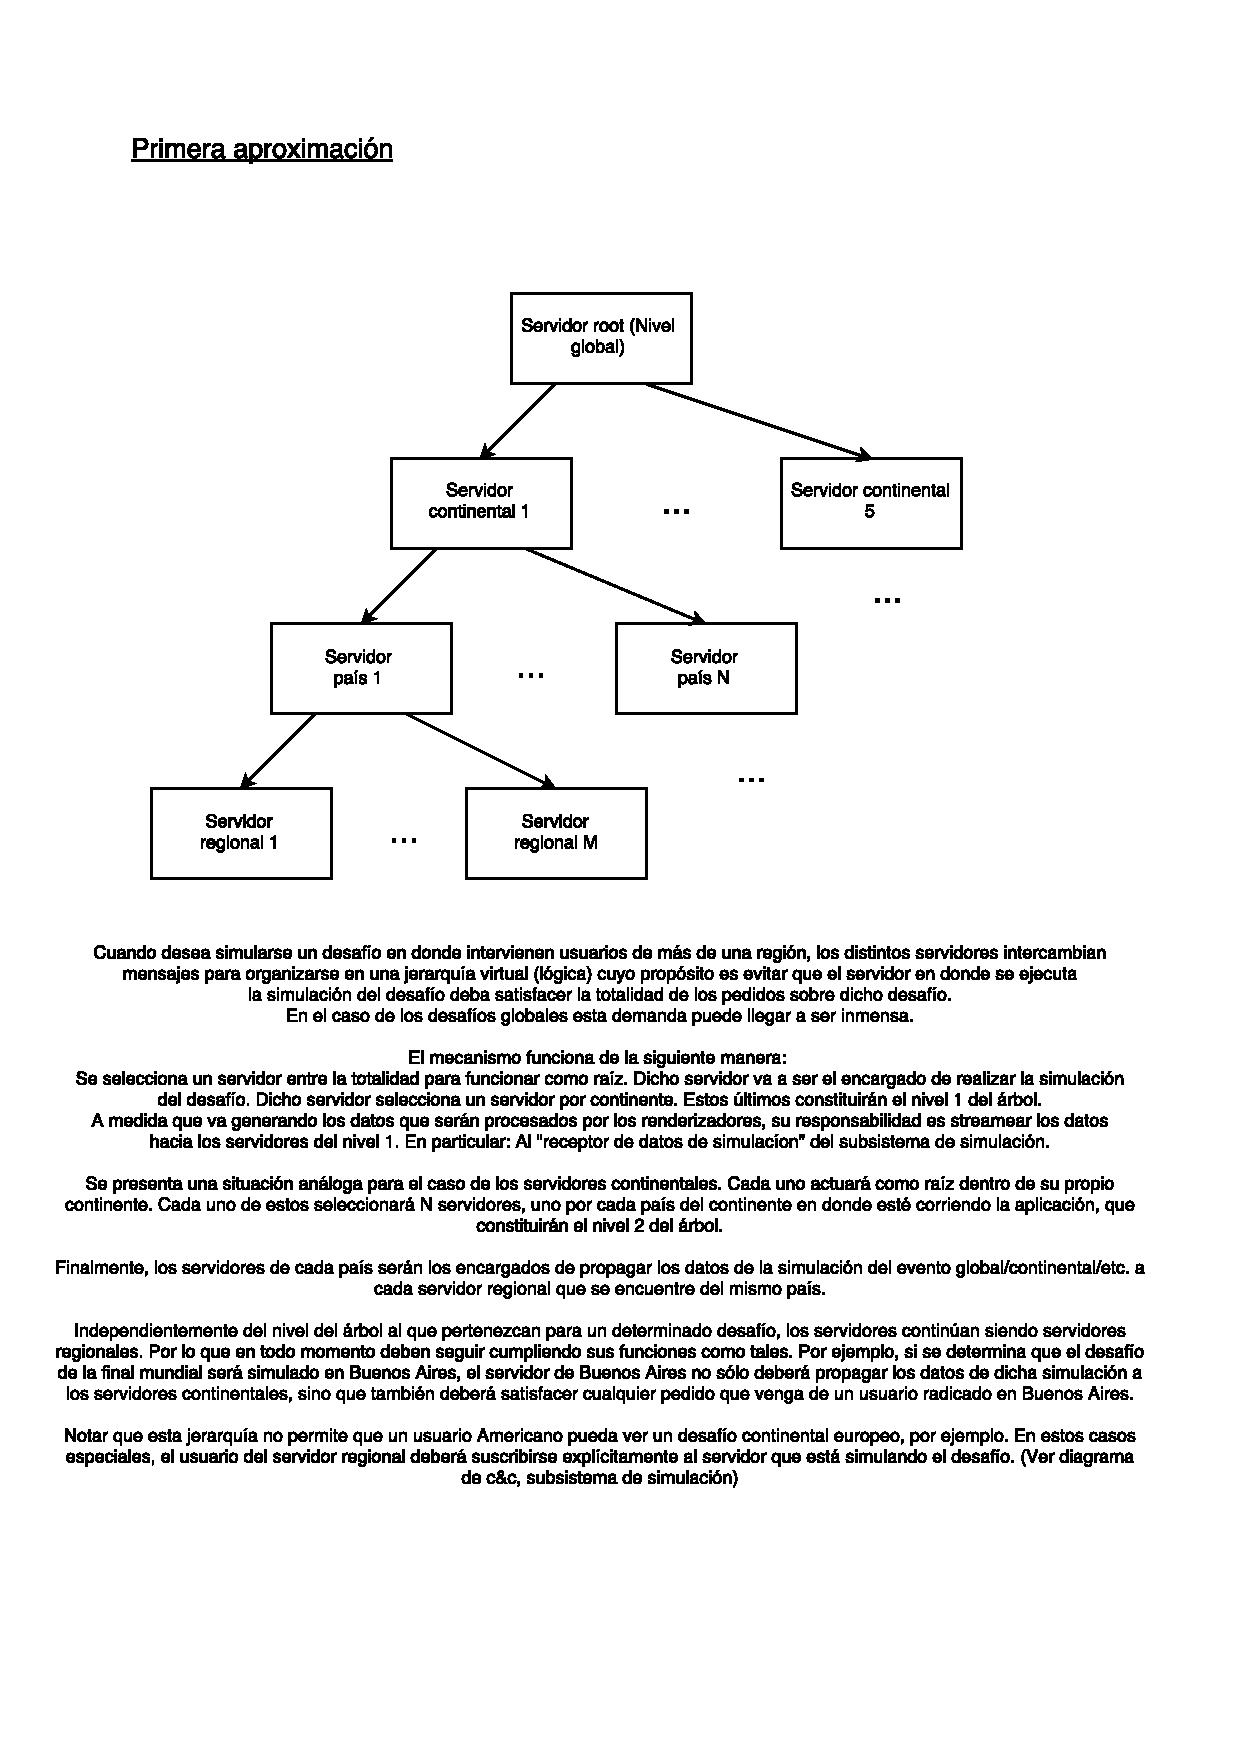
\includegraphics[width=\textwidth, page=1, clip, trim=20 0 20 110]{imagenes/jerarquia-global.pdf}
\end{figure}
\newpage
\begin{figure}[H]
  \includegraphics[width=\textwidth, page=2, clip, trim=20 20 20 10]{imagenes/jerarquia-global.pdf}
\end{figure}

\begin{figure}[H]
  \centering
  \includegraphics[width=\textwidth]{imagenes/nivel1-simulaciones.png}
\end{figure}

\newpage

\subsection{Subsistema de Desafios}
\begin{figure}[H]
  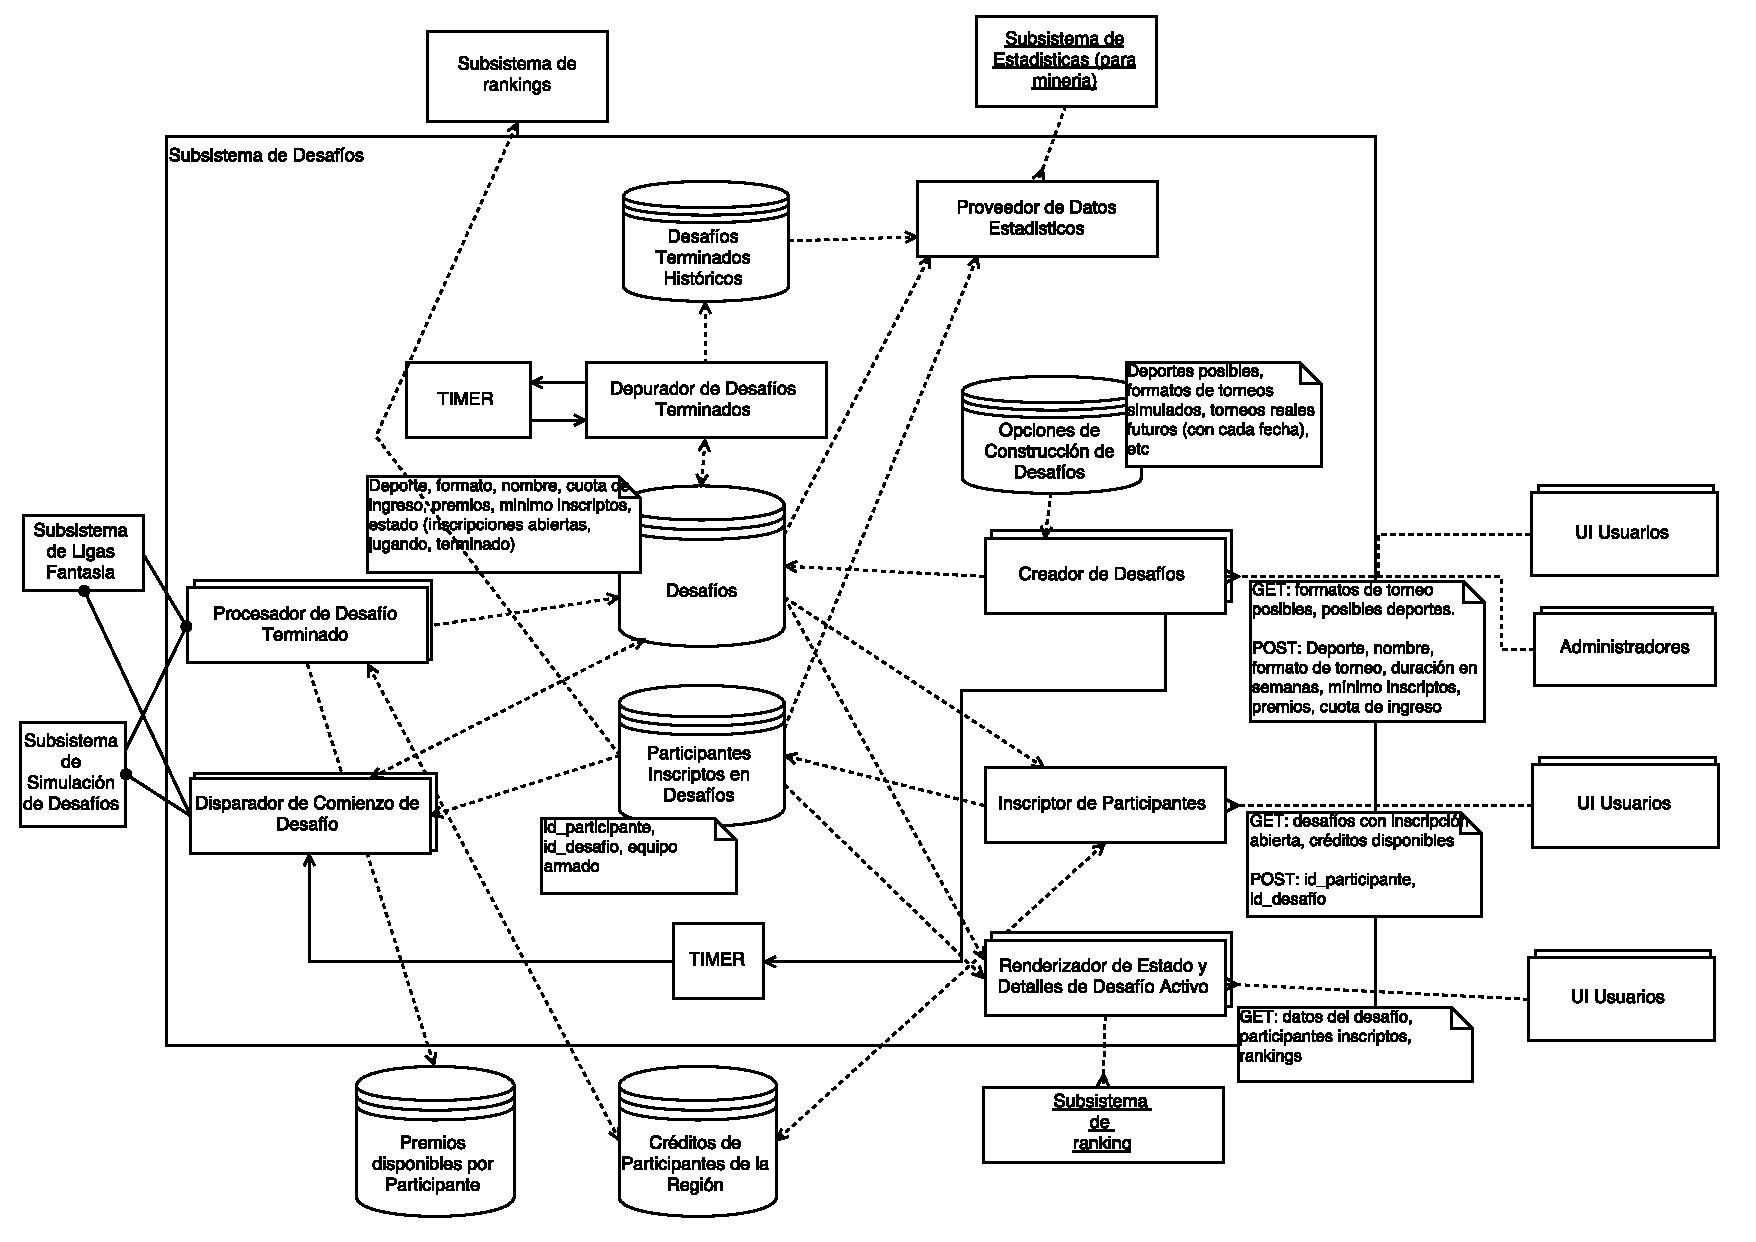
\includegraphics[width=1.1\textwidth, page=1, clip, trim=10 0 10 0]{imagenes/Subs-desafios.pdf}
  \caption{Subsistema de Desafios.}
\end{figure}
% \newpage
El subsistema de desafíos se encarga de crear desafíos, inscribir participantes, iniciar desafios en el momento indicado, proveer detalles y estado de cada desafio a los usuarios.
Cuando un desaífo comienza se encarga de informar al subsistema de simulación o liga de fantasia seúgn corresponda. Además se encarga de cobrar créditos de inscripción y de pagar premios (tanto en créditos como premios especiales, que luego los usuarios podrán cambiar por el premio real en dinero o lo que corresponda. También provee una interfaz de consulta de estadísticas de desafios.\\

\begin{itemize}
\item Desafíos Terminados: Los desafíos finalizados durante la última semana van a tener más solicitudes de consulta de estado. Es por esto que esos desafíos se mantienen
en el repositorio principal de desafíos con redundancia activa para mejorar la disponibilidad y la performance. Pasados los 7 días de finalizado, un proceso que ejecuta una vez por día se encarga de depurar el repositorio principal para mejorar la performance de las búsquedas, asumiendo que esos desafíos serán consultados con menos frecuencia.

\item Creador de Desafíos: Devuelve todas las opciones posibles para construir un desafío (tanto para modo simulado como para modo liga de fantasía). Luego recibe la configuración elegida y crea el desafío. Se almacena en un repositorio local que luego se propaga a todas las réplicas regionales.

\item Inscripción de participantes: Muestra una lista con todos los desafíos por cada deporte (tanto simulados como liga de fantsía) que aún estén con la inscripcion abierta (aún no comenzaron ajugarse). Por cada uno muestra el valor en creditos para ingresar. Luego se inscribe un participante (siempre y cuando ls créditos le alcancen). Para mejorar la performance y disponibilidad (muchos podíran intentar inscribirse a la vez), luego de hacer el checkeo se guardan en una caché todos los pedidos de  inscripcion que luego se van persistiendo por procesos dedicados.

\item Renderizador de estado y detalles: Devuelve el estado de un desafio especifico (si está abierto a inscripciones, si se esta jugando o si está terminado) asi como también la cuenta regresiva para que empiece el desafio (y se cierren inscripciones) y todos los detalles asociados (premios, cuota de inscripción, tipo de desafío, formato de torneo o fechas que se juegan, etc.), y el ranking, si corresponde. Internamente se utiliza una caché. Cada pedido que llega se guarda en un repositorio y se solicitan los datos a un manager de cache (que se crea en el momento que se necesita) y a un proceso que busca los datos en los repositorios persistentes (tambéin se crea cuando se necesita). Si el dato llega de la caché, se mata al proceso que  fue a disco (y tambien se mata al proceso de la caché). En cambio si no estaba en la caché, el dato llegaár del disco (y ahí tambéin se guarda en la caché para soportar eficentemente un período corto de muchos pedidos de detales del mismo desafio. Un proceso se ejecuta cada 1 minuto y borra los datos de caché que tengan más de un minuto de antigüedad. Dado que los datos no deben mostrarse en tiempo real, este mcanismo mejora la disponibildad y la performance de respuesta a muchas solicitudes de detalles de un desafío popular.
\end{itemize}

\begin{figure}[H]
  \includegraphics[width=\textwidth, page=3, clip, trim=20 0 20 30]{imagenes/Subs-desafios.pdf}
  \caption{Zoom en Procesador Desafio Terminado y Creador de Desafios}
\end{figure}

\begin{figure}[H]
  \includegraphics[width=\textwidth, page=4, clip, trim=20 0 20 0]{imagenes/Subs-desafios.pdf}
  \caption{Zoom en Inscriptor de Participantes y Renderizador de Estados y Detalles Desafio Activo}
\end{figure}

\newpage

\subsection{Subsistema de Simulacion}
\begin{figure}[H]
  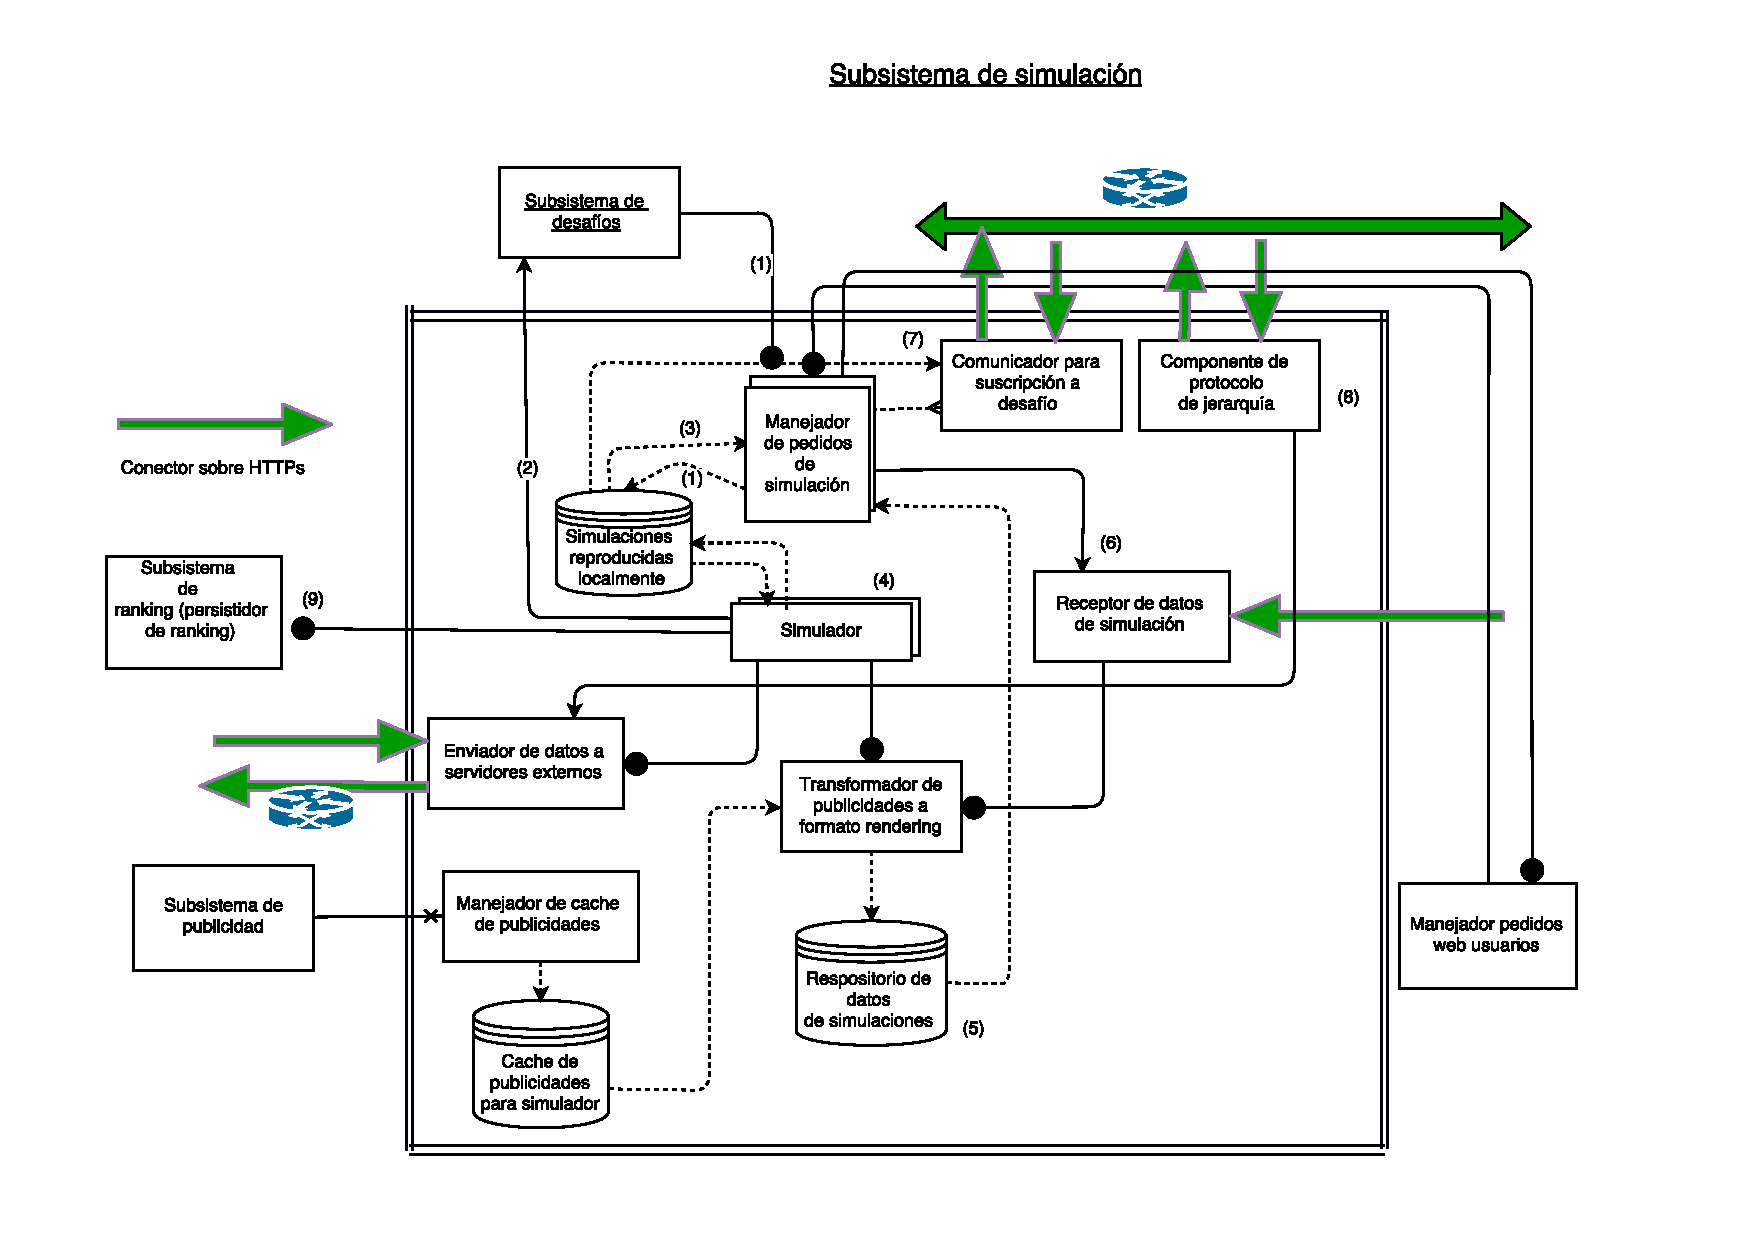
\includegraphics[width=1.1\textwidth, page=1, clip, trim=10 0 10 0]{imagenes/subs-simulacion.pdf}
  \caption{Subsistema de Simulacion.}
\end{figure}

\begin{figure}[H]
  \includegraphics[width=1.1\textwidth, page=2, clip, trim=25 0 10 0]{imagenes/subs-simulacion.pdf}
  \caption{Enviador Datos a servidores externos.}
\end{figure}

\begin{figure}[H]
  \includegraphics[width=1.1\textwidth, page=3, clip, trim=25 250 10 0]{imagenes/subs-simulacion.pdf}
  \caption{Receptor de datos de Simulacion.}
\end{figure}

\newpage

\subsection{Subsistema de Ligas de Fantasia}
\begin{figure}[H]
  \centering
  \includegraphics[width=\textwidth]{imagenes/fantasia.png}
  \caption{Subsistema de Ligas de Fantasia.}
\end{figure}

El procesador de comienzo de desafío almacena el desafío nuevo en el repositorio de desafíos activos, junto con todos los partidos a tener en cuenta.
Luego crea un procesador de comienzo de partido, que se encarga de revisar si el desafío indicado tiene algún partido que comenzar, y en caso que no sea así, programa un timer para
que le avise cuándo comienza el próximo partido. En este esquema, se crea un procesador de comienzo de partido para cada desafío nuevo que llega.
Cada vez que hay un partido, el procesador de comienzo de partido crea un procesador de minuto a minuto de partido. Este último, cada un minuto,
solicita al Subsistema de Estadisticas de Partidos las últimas actualizaciones. Con ellas evalúa las reglas de puntajes y actualiza los rankings (por ejemplo, una regla podría ser "Si mete gol, suma 3 puntos", y si una actualización
indica que Agüero metió un gol, entonces se envia al ranking A todos los participantes cuyo equipo tenga a Agüero suma 3 puntos).
Una vez actualizado los rankings, vuelve aprogramar el timer por un minuto. De esta manera habrá un procesador minuto a minuto por cada partido activo, que en cada minuto
actualizará los puntajes del ranking.\\

El procesador de comienzo de partido, luego de crear el de minuto a minuto, se programa
para el próximo partido. Si no hay más partidos, simplemente se destruye a sí mismo.\\

Cuando cada partido termina, el procesador de minuto a minuto se destruye a sí mismo, pero antes avisa del fin de partido al procesador de fin de partido, que verifica si
fue el último del desafio y en tal caso informa de la finalización del partido al subsistema de desafíos.

\newpage

\subsection{Subsistema de Ranking}
\begin{figure}[H]
  \centering
  \includegraphics[width=\textwidth]{imagenes/Subsistema-ranking.png}
  \caption{Subsistema de Rankings.}
\end{figure}

\newpage

\subsection{App Cliente}
\begin{figure}[H]
  \centering
  \includegraphics[width=\textwidth]{imagenes/Cliente.png}
  \caption{Applicacion del lado del Cliente.}
\end{figure}

\newpage

\subsection{Manejador pedidos Cliente}
\begin{figure}[H]
  \centering
  \includegraphics[width=\textwidth]{imagenes/Manejador-de-pedidos.png}
  \caption{Manejador de pedidos realizados por el cliente.}
\end{figure}

\newpage

\subsection{Subsistema de Usuarios}
\begin{figure}[H]
  \centering
  \includegraphics[width=\textwidth]{imagenes/manejo-usuarios.png}
  \caption{Subsistema de manejo de usuarios.}
\end{figure}

Cuando un usuario se registra, el manejador
ingresa la información en la base de datos.
Para interactuar con el sistema, el usuario
inicia una sesión.
Ante cada pedido, el sistema autoriza que el
usuario que generó el pedido tenga suficientes
permisos para hacerlo

\newpage

\subsection{Subsistema de Cobro y Pagos}
\begin{figure}[H]
  \centering
  \includegraphics[width=\textwidth]{imagenes/subs-cobro-y-pago.png}
  \caption{Subsistema de cobros y pagos.}
\end{figure}

Los datos de tarjetas y cuentas y el Tokenizador corren en una maquina distinta a todo el resto. Esto se hace para aislarla lo maximo posible y evitar cualquier vulnerabilidad que pueda llegar a tener el resto del sistema. Ademas estas maquinas deberan tener seguridad fisica, para evitar posibles robos y/o violaciones fisicas al sistema.

Funcionamiento:
\begin{enumerate}
\item {
  \begin{itemize}
  \item Caso medio de pago nuevo:
  Al manejador le llegan pedidos de pagos y/o cobros, autenticados y con informacion de un medio de pago nuevo. Entonces le pasamos esta informacion a el Tokenizador, que le genera un token, persiste en base de datos la informacion y el token correspondiente y le devuelve el token al Manejador de pedidos.
  \item Caso medio de pago existente:
  Al manejador le llegan pedidos de pagos o cobros, autenticados y con un id o refencia minima (elegida en por el Cliente) de que medio de pago se usara. Entonces con ese id o referencia, le pedimos al Tokenizador y obtenemos el token correspondiente.
  \end{itemize}
}

\item Luego con el token correspondiente, se lo brindamos al Realizador de pedidos, que entiende de tokens y con el se comunica con el medio de pago correspondiente y realiza la accion pertinente brindandole el token al medio de pago.

\item Luego con el resultado de la accion, la logeamos en el registro de movimiento y le devolvemos el resultado de la accion al Realizador y este al Manejador
\end{enumerate}

Ademas la información mas sensible (Numero de Tarjeta o Cuenta completa, codigo de seguridad de la tarjeta, etc) seran almacenada encriptada, mediante un algoritmo de clave asimetrica, donde la clave para desencriptar la tengan unicamente los dueños del sistema.

De esta forma, cumpliriamos con un estandar de seguridad llamado PCI, el cual es necesario para para poder realizar cobros y pagos con tarjetas de credito y cuentas bancarias. Este estandar sera todo el tiempo testeado para verificar que estemos siempre cumpliendo y en norma, ya que en caso de no estarlo estariamos abierto a posibles ataques y/o robos de datos.

\subsubsection{Biografia consultada}
\begin{itemize}
\item \href{https://www.pcisecuritystandards.org/documents/Tokenization_Guidelines_Info_Supplement.pdf}{Norma PCI.}\\
\item \href{https://www.quora.com/Do-companies-like-Amazon-etc-have-a-server-farm-to-store-creditcard-information-on-database}{Como cuidan sus datos compañias del estilo Amazon.}
\end{itemize}

\newpage

\subsection{Subsistema de Streaming}
\begin{figure}[H]
  \centering
  \includegraphics[width=\textwidth]{imagenes/subs-streaming.png}
  \caption{Subsistema de streaming de partidos reales.}
\end{figure}

La interacción entre el manejador de pedidos y el componente de streaming de partidos reales es análoga al de las simulaciones.
Los usuarios envían un pedido al manejador en donde solicitan ver el partido 'i'.
El manajador guarda una entrada en el repositorio en donde agrega una entrada que establece que el usuario 'u' está subscripto
al streaming del partido 'i'.

El manager de pedidos de streaming crea entonces una entrada en el 'repositorio de streams solicitados'. Este repositorio es 
consultado por el receptor de desafíos para saber a qué streamings generados por los proveedores de transmisiones suscribirse. 

Hay un conector custom por cada proveedor de servicios diferente

\newpage

\subsection{Subsistema de Publicidad}
\begin{figure}[H]
  \centering
  \includegraphics[width=\textwidth]{imagenes/Subsistema-de-publicidad.png}
  \caption{Subsistema de Publicidades.}
\end{figure}

La idea es que el manejador de pedidos stakeholders le indique al persisitidor de publicidades qué publicidad desea
guardar, indicándole en dónde deber mostrarse (transmisión de un partido, simulación o página principal del sitio) y en qué momento (hora).
Luego, el obtenedor de publicidades consulta periodicamente (cada 3 segundos) el repositorio solicitándole publicidades que deban mostrarse
en el momento en que consulta (+/- 3 segundos) y las envía a traves de un router a cada componente que hará uso del mismo (subsistema de
 simulación, subsistema de streaming y manejador de pedidos de usuario)

\newpage

\subsection{Subsistema de Estadisticas de Partidos}
\begin{figure}[H]
  \centering
  \includegraphics[width=\textwidth]{imagenes/Subsistema-de-estadistica-de-partido.png}
  \caption{Subsistema de Estadisticas de Partidos.}
\end{figure}

Los proveedores estadisticos que tenemos contratados publican actualizaciones periodicas de los partidos que se están disputando.
Como los datos publicados son propensos a errores decidimos utilizar un voter central que recibe las salidas de los múltiples procesadores y decide el
resultado correcto en función de los votos. Estos resultados son persisitidos en un repositorio el cual puede ser accedido mediante el obtenedor de
estadísticas de partidos.

\newpage



\newpage

\bibliographystyle{plain}
\bibliography{tp3}

\end{document}
